\chapter{Développement logiciel}

Ce chapitre a pour but d'expliquer l'implémentation logicielle sur les 3 plateformes utilisées (DevBox, Android et le serveur en Python). L'architecture générale y est présentée, mais également les implémentations spécifiques à chaque sous-catégorie.


\section{Architecture générale}

\begin{figure}[ht!]
    \centering
    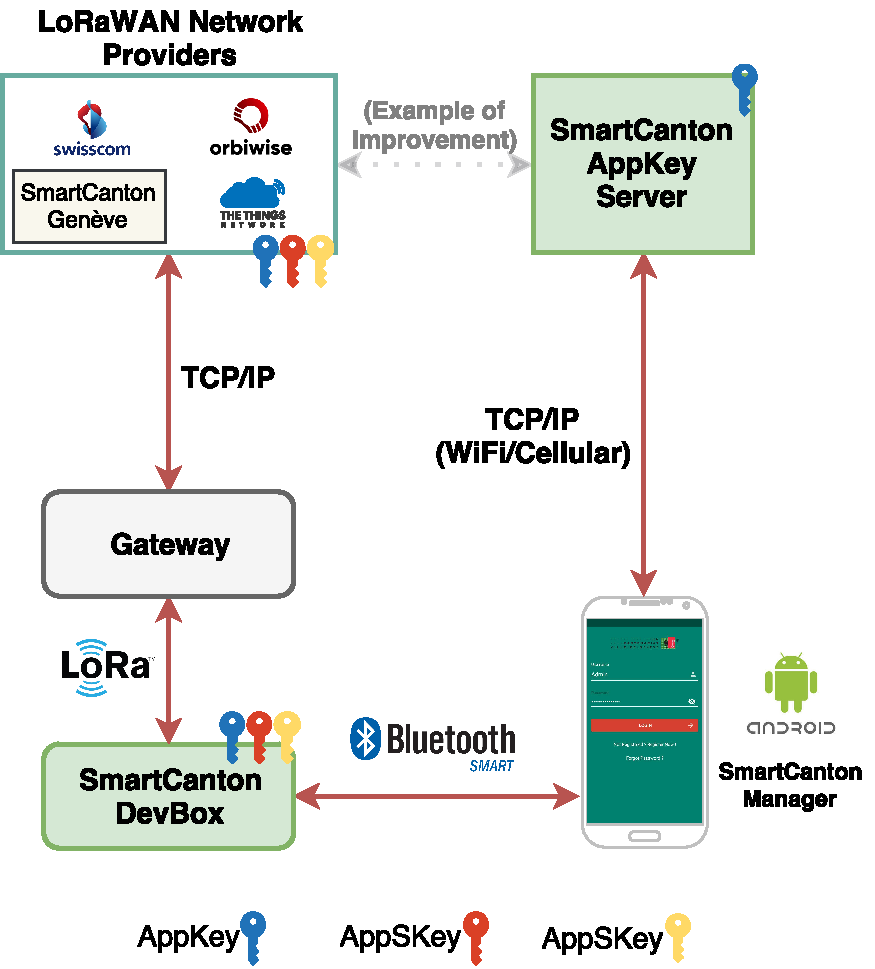
\includegraphics[width=0.7\textwidth]{Figures/Software/diagram_project_software.pdf}
    \caption{Schéma général du projet avec les différentes technologies utilisées}
    \label{fig-diagram_project_software}
\end{figure}

L'architecture logicielle avec les différents protocoles de communications est visible sur la \cref{fig-diagram_project_software}. Au centre se situe la DevBox qui a deux interfaces de communication avec le LoRa et le Bluetooth Low Energy. Le Bluetooth sera accessible par une application développée pour Android dans un premier temps. La DevBox implémente une table GATT pour les services liés à la DevBox (batterie, LoRaWAN, GPS, BME680, etc. ). Ceux-ci sont explorés en détail en \cref{sec-BLEAllServices}.



\section{Scanneur de périphériques Bluetooth Low Energy}
\label{sec-software_scanner_ble}

L'implémentation du scanner de périphériques Bluetooth Low Energy est à cheval sur deux plateformes (Android et DevBox). Les spécifications liées à l'implémentation sur les plateformes sont présentées dans leurs sections respectives (\cref{sec-soft_devbox} et \cref{sec-soft_android}). \\


Les spécificités des \textit{advertisements} BLE ont été présentées dans l'état de l'art de ce document (\cref{sec-stateoftheart_ble}). Lorsqu'un périphérique Bluetooth Low Energy souhaite être visible, il doit diffuser un paquet de données. Ce paquet est entièrement personnalisable par l'utilisateur. Trois types de \textit{beacons} ont été présentés, parmi ceux-là, l'AltBeacon a été l'implémentation choisie. Principalement parce qu'elle est plus libre que le iBeacon. En effet, les \textit{Manufacturer ID} ne sont pas délivrés par une entité, contrairement aux iBeacons (si on souhaite être certifiée
par Apple). L'Eddystone est aussi très personnalisable, mais son grand avantage provient de ses URLs, qui dans notre projet ne sont pas nécessaires.  \\

Le \cref{tab-AltBeaconSmartCantonFormat} explique le contenu du format choisi pour diffuser la position. L'UUID de 16bit a un \textit{pattern} similaire à celui choisi pour les services Bluetooth. Ce qui est intéressant de voir c'est les bytes pour le Major et le Minor. Ceux-ci sont générés une seule fois aléatoirement pour chaque client au lancement du diffuseur d'\textit{advertisements}. Cela permet ainsi de traquer un utilisateur durant un laps de temps contrôlable, c'est-à-dire, tant que l'application n'est pas arrêtée sur le périphérique. L'adresse MAC du Bluetooth peut donc changer, mais on pourra suivre un utilisateur simplement en sauvegardant ce paquet.


\begin{table}[ht!]
\centering
\caption{Format du AltBeacon utilisé par le scanner Bluetooth}
\label{tab-AltBeaconSmartCantonFormat}
\begin{tabular}{|l|c|c|c|c|}
\hline
\multicolumn{5}{|c|}{\cellcolor[HTML]{BBDAFF}\textbf{AltBeacon Template}} \\ \hline
\textbf{Byte} & \textbf{0} & \textbf{1} & \textbf{2} & \textbf{3} \\ \hline
\textbf{0} & AD Length & AD Type & \multicolumn{2}{c|}{MFG ID} \\ \hline
\textbf{32} & \multicolumn{2}{c|}{BEACON Code} & \multicolumn{2}{c|}{BEACON ID} \\ \hline
\textbf{64} & \multicolumn{2}{c|}{BEACON ID} & \multicolumn{2}{c|}{BEACON ID} \\ \hline
\textbf{96} & \multicolumn{2}{c|}{BEACON ID} & \multicolumn{2}{c|}{BEACON ID} \\ \hline
\textbf{128} & \multicolumn{2}{c|}{BEACON ID} & \multicolumn{2}{c|}{BEACON ID} \\ \hline
\textbf{160} & \multicolumn{2}{c|}{BEACON ID} & \multicolumn{2}{c|}{BEACON ID} \\ \hline
\textbf{192} & \multicolumn{2}{c|}{BEACON ID} & RSSI TX & MFG RSV \\ \hhline{=====}
\multicolumn{5}{|c|}{\cellcolor[HTML]{BBDAFF}\textbf{AltBeacon SmartCanton}} \\ \hline
\textbf{Byte} & \textbf{0} & \textbf{1} & \textbf{2} & \textbf{3} \\ \hline
\textbf{0} & 0x1B & 0xFF & 0xFF & 0xFF \\ \hline
\textbf{32} & 0xBE & 0xAC & 0x00 & 0x00 \\ \hline
\textbf{64} & 0x00 & 0x00 & 0xAA & 0xAA \\ \hline
\textbf{96} & 0xBB & 0xBB & 0xCC & 0xCC \\ \hline
\textbf{128} & 0xDD & 0xDD & 0xDD & 0xDD \\ \hline
\textbf{160} & 0xDD & 0xDD & \multicolumn{2}{c|}{RANDOM} \\ \hline
\textbf{192} & \multicolumn{2}{c|}{RANDOM} & 0xBB & 0x00 \\ \hline
\end{tabular}
\end{table}


% ----------------------------------------------------------------- %
\FloatBarrier
\FloatBarrier
\newpage
\section{DevBox : module LoRaWAN}
\label{sec-soft_devbox}


Le module LoRaWAN est interconnecté avec le microcontrôleur Bluetooth via une interface UART. Le débit final de cette interface a été fixé à 115200 bits 
par seconde.

\subsection{Architecture logicielle}


STMicroelectronics propose une suite de bibliothèques pour ses divers microcontrôleurs afin de pouvoir communiquer avec des modules LoRa. Cette suite de bibliothèques est basée sur la très connue suite de développement STM32Cube\footnote{\url{http://www.st.com/en/embedded-software/stm32cube-mcu-packages.html}} et nommé \texttt{STM32 LoRa software expansion} \cite{STM32LoR36:online}. La \cref{fig-murata_lorawan_architecture} illustre l'architecture logicielle de cette suite de bibliothèques. Elle est composée d'un Hardware Abstraction Layer avec tous \textit{drivers} des périphériques du microcontrôleur STM32. Pour le \textit{middleware}, les blocs en vert sont repris de Semtech avec leur projet LoRaMac-node\footnote{\url{https://github.com/Lora-net/LoRaMac-node}}, alors que les blocs en bleu sont les \textit{drivers} fournis par ST. Il s'agit là de \textit{drivers} qui sont uniquement utilisés sur les différents capteurs présents sur les cartes de développement, telles que la B-L072Z-LRWAN1 et donc non utilisée dans ce projet. Il a un bloc nommé \textit{utilities}, créé par Semtech, mais modifié par ST. Cette modification permet d'utiliser au mieux les ressources matérielles du STM32L0, telles que les \textit{timers}, le mode \textit{Low-Power}, ainsi que le \textit{True Random Number Generator} (TRNG). L'architecture complète de cette suite de bibliothèques, ainsi que la description des diverses fonctions sont décrites dans le manuel d'utilisateur numéro \textbf{UM2073} de ST \cite{STM32LoR36:online}. 

\begin{figure}[ht!]
    \centering
    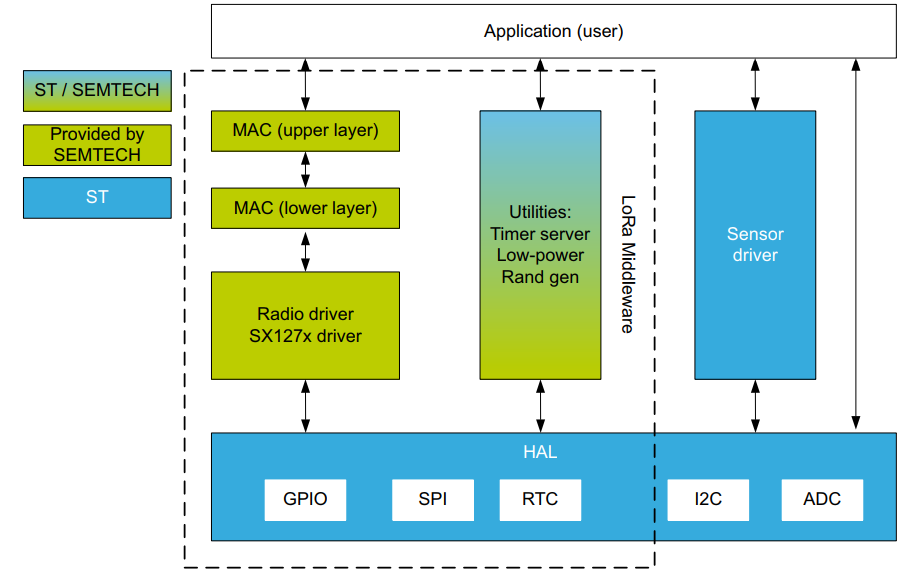
\includegraphics[width=0.8\textwidth]{Figures/Software/LoRaWAN/murata_lorawan_architecture.png}
    \caption{Architecture logicielle du CMWX1ZZABZ}
    \label{fig-murata_lorawan_architecture}
\end{figure}



\subsection{Exemples et modifications}
STMicroelectronics propose trois exemples de codes pour le CMWX1ZZABZ adaptés pour la carte de développement B-L072Z-LRWAN. Voici la description de ces projets : 
\begin{enumerate}
    \item \texttt{End Node} : projet ayant pour but de créer un n\oe ud LoRaWAN autonome avec la possibilité d'envoyer des données à des intervalles réguliers ou lors de la pression d'un bouton. 
    
    \item \texttt{AT Master} : offre la possibilité de communiquer avec un nouveau coprocesseur LoRa, implémentant un AT Slave interface. Cet exemple est très complet et est très utile pour comprendre comment la communication avec un AT Slave fonctionne. La \cref{fig-at_slave_master_connection} illustre la connexion entre un microcontrôleur utilisant l'interface \textit{Master} et un \textit{Slave}. Néanmoins, ce projet repose sur beaucoup de bibliothèques de ST, il est donc difficile de l'utiliser directement sur un microcontrôleur d'un autre fabricant.
    
    \item \texttt{AT Slave} : est utilisé pour offrir une interface de programmation du module à un utilisateur. Cet utilisateur peut utiliser un simple terminal série afin d'envoyer des commandes AT ou directement connecter un microcontrôleur (cf. \cref{fig-at_slave_master_connection}). La liste de toutes les commandes AT est disponible dans la note d'application nommée AN4967\footnote{\url{www.st.com/resource/en/application_note/dm00346311.pdf}}, avec les paramètres, ainsi que les réponses.
\end{enumerate}


\begin{figure}[ht!]
    \centering
    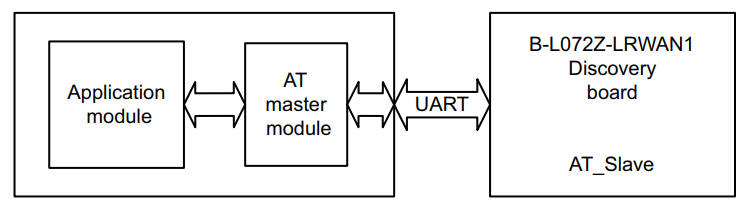
\includegraphics[width=0.7\textwidth]{Figures/Software/LoRaWAN/at_slave_master_connection.png}
    \caption{Connexion entre un AT \textit{Slave} et un AT \textit{Master} utilisant la suite de bibliothèque STM32Cube LoRa}
    \label{fig-at_slave_master_connection}
\end{figure}

Une interface entre le KW41Z et le CMWX1ZZABZ doit être implémentée, il a donc été décidé de reprendre le projet AT Slave pour le CMWX1ZZABZ et de l'adapter au besoin de la carte. Cet exemple implémente déjà toutes les opérations nécessaires pour rejoindre un réseau LoRa et envoyer des données. Le seul inconvénient de cette interface est l'utilisation d'un protocole basé sur des strings qui demande plus de stockage en mémoire et de temps pour transformer les requêtes. Mais le KW41Z a 128 kB de RAM, qui sont amplement suffisants pour cela. Toutefois, le code a dû être modifié avant d'enlever quelques périphériques qui ne sont pas présents sur la DevBox. Il faut également changer l'interface de communication afin d'utiliser l'UART0 de la carte qui n'est pas sur les mêmes pins que le LPUART initialement connecté.



\section{DevBox : NXP Kinetis KW41Z}

Le développement logiciel du microcontrôleur NXP Kinetis KW41Z est l'élément central de ce projet. Il implique l'interfaçage de divers périphériques avec plusieurs interfaces distinctes et tout cela sur un système temps réel.  

% ---------------------------------------------------------------------------------------------%
\subsection{\textit{OS Abstraction Layer} et \textit{Connectivity Framework}}
% ---------------------------------------------------------------------------------------------%

Les exemples de codes fournis par NXP pour ses microcontrôleurs implémentent tous FreeRTOS. Comme présenté en \cref{sec-RTOS_freertos}, il s'agit actuellement du RTOS le plus populaire et le plus actif en termes de communauté, ce qui apporte beaucoup d'avantages lors du développement. Lors de la présentation des différents RTOS, il a été fait référence aux couches d'abstraction de RTOS, en prenant l'exemple de l’OS Abstraction Layer (cf. \cref{sec-rtos_abstract_layer}). Celui-ci est visible sur la \cref{fig-freescale_osa_framework}. Il offre ainsi la possibilité de changer facilement de RTOS en fonction des besoins du projet pour les utilisateurs. NXP propose un framework nommé \textit{Connectivity Framework} qui s'occupe principalement des connexions avec le monde extérieur (Bluetooth, Wifi, etc.), mais également qui incluent différents autres blocs qui sont tous affichés sur la \cref{fig-freescale_osa_framework}. 

\begin{figure}[ht!]
    \centering
    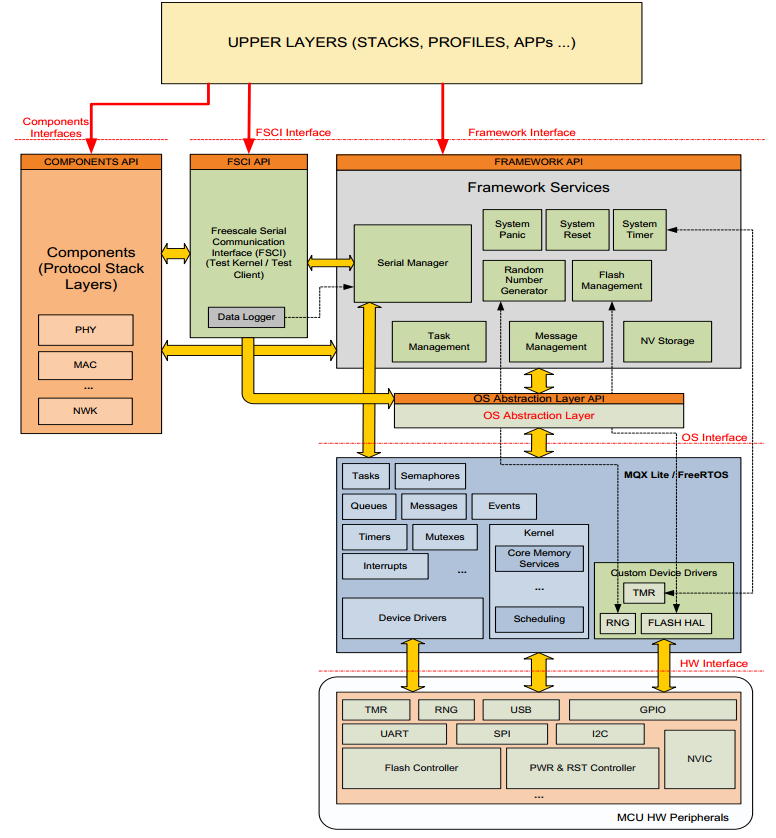
\includegraphics[width=1.0\textwidth]{Figures/Software/freescale_osa_framework.PNG}
    \caption{\textit{Connectivity Framework} de Freescale (NXP)}
    \label{fig-freescale_osa_framework}
\end{figure}

Tout d'abord, en commençant par les différents blocs en bas de la \cref{fig-freescale_osa_framework} , la présence de plusieurs \textit{drivers} pour les périphériques peut être constatée. Ceux-ci couvrent toutes les interfaces de communications présentes sur les microcontrôleurs et sont tous très complets. On a ensuite la présence d'un RTOS qui est composé des différents composants standards d'un RTOS tel que des \textit{queues}, sémaphores et mutexes. Cette couche de RTOS repose directement sur l'interface matérielle, car il est parfois nécessaire d'adapter les drivers pour qu'ils soient \textit{thread safe} en fonction des différents ordonnancements utilisés par les RTOS et ainsi garantir l'intégrité des données. Vient ensuite l'interface OS Abstraction Layer pour uniformiser les différents RTOS. Un certain nombre de services sont disponibles, comme par exemple, le \textit{Serial Manager} qui a été utilisé dans ce projet pour gérer les connexions UART avec le coprocesseur LoRa. Celui-ci peut gérer des flux asynchrones provenant de plusieurs types d'interfaces (UART, USB, I2C et SPI). Pour les interfaces I2C ou SPI, celles-ci doivent être configurées avec une interruption sur un GPIO pour informer le \textit{Serial Manager }qu'une nouvelle donnée est disponible. La plupart de ces frameworks sont des tâches RTOS propre et utilisent des interfaces de communications \textit{thread-safe} afin d'être programmés.  \\

Ensuite, on peut voir l'élément qui simplifie l'intégration des communications externes (Bluetooth, WiFi, etc.) qui se nomme \textit{Components API}. Ce bloc a pour but de faciliter la programmation des diverses \textit{stacks} présentes sur les microcontrôleurs en fonctions des différentes gammes. On retrouve ainsi le Bluetooth, mais également des stacks pour le TCP/IP ou Thread. C'est souvent ce dernier bloc qui n'est pas open source. \\

\textit{Freescale Serial Communication Interface} (FSCI) est à la fois un module, mais également un protocole de communication utilisé entre les interfaces de communications externes (\textit{Components API}) et les services. On peut voir sur la \cref{fig-freescale_osa_framework} qu'il n'est pas forcément nécessaire de passer par le FSCI pour accéder aux composants depuis les composants applicatifs. Le FSCI ainsi que les \textit{frameworks} Services sont documentés dans un manuel de référence de NXP nommé \texttt{CONNFWKRM}. Toutefois, la documentation est légère, il est souvent plus facile de regarder le code source ou simplement les fichiers d'entêtes de fonctions pour les parties non open sources.

Le bloc, le plus haut niveau du framework, nommé \textit{upper layers}, est là où l'utilisateur doit normalement implémenter la plus grande partie de son code. Il a ensuite accès à ses trois interfaces pour utiliser toutes les ressources à sa disposition sur le microcontrôleur.


% ---------------------------------------------------------------------------------------------%
\FloatBarrier
\subsection{Interfaces de programmation}
% ---------------------------------------------------------------------------------------------%


\begin{figure}[ht!]
    \centering
    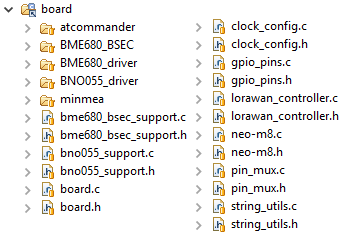
\includegraphics[width=0.6\textwidth]{Figures/Software/kw41z/board_paths.png}
    \caption{Bibliothèques et \textit{drivers} utilisés sur la DevBox}
    \label{fig-board_paths}
\end{figure}

Lors du développement de ce projet, plusieurs éléments ont été utilisés afin de simplifier la programmation de la DevBox. Un répertoire nommé \path{smartcanton_devbox_board} présent dans le dépôt GitHub au chemin d'accès, \path{dev/MKW41Z} contient des interfaces qui ont pour but d'être utilisées sur tous les projets qui utiliseront la DevBox à l'avenir. Ce répertoire est ensuite ajouté à l'aide d'un lien symbolique dans le projet MCUXpresso, comme illustré à l'aide de la \cref{fig-board_paths}. Certains de ces éléments sont des bibliothèques ou \textit{drivers} qui ont été développés par la communauté ou directement par les fabricants des composants électroniques utilisés.


\subsubsection{Bibliothèques et \textit{drivers} repris}

En plus du SDK fourni par NXP avec les différents \textit{drivers} pour le KW41Z, un certain nombre de bibliothèques ont été reprises et utilisées afin d'accélérer le développement du projet.

\subsubsubsection{AT Commander}
\label{sec-software_libs_atcommander}
La communication avec le module LoRaWAN s'effectue avec des commandes AT. Pour cela, une bibliothèque nommée AT Commander a été utilisée : 
\begin{center}
    \url{https://github.com/openxc/AT-commander}
\end{center}

Elle a toutefois du être modifiée à cause du format des requêtes qui sont transmissent par le module LoRaWAN. Cette bibliothèque est par défaut utilisable avec des modules AT de type RN42 ou XBEE, dont le format de trames diffère de celles du projet STM32 LoRa. Pour utiliser cette bibliothèque, l'utilisateur doit simplement spécifier deux fonctions pour lire et écrire sur un port UART souhaité. 

\subsubsubsection{minmea}
\label{sec-software_libs_minmea}

Le \textit{parsing} des trames GPS est fastidieux et peut être complexe en fonction des différents GPS et du type de données contenues dans une trame GPS. Il existe beaucoup de bibliothèques pour les GPS, mais souvent celles-ci ne sont pas adaptées aux systèmes embarqués. Cela s'explique par les fonctions de traitement de \textit{strings} qui demandent trop de ressources au processeur. Heureusement, il existe une bibliothèque nommée \texttt{minmea} qui implémente un parseur pour la spécification NMEA 0183 \cite{NMEA018318:online}. Celle-ci est pensée pour les environnements avec des capacités restreintes, comme les microcontrôleurs. Elle est disponible à l'adresse suivante :

\begin{center}
    \url{https://github.com/kosma/minmea}
\end{center}

\texttt{Minmea} est composée de deux fichiers et très simple d'utilisation. La trame récupérée depuis le GPS lui est directement fournie et celle-ci s'occupe d'extraire toutes les informations souhaitées. Elle supporte les données de type RMC, GGA, GSA, GLL, GST, GSV, VTG et ZDA \cite{NMEAdata3:online}. Toutes les données sont ensuite accessibles via des structures selon le type de données.

\subsubsubsection{BNO055 \textit{driver}}
\label{sec-softwaire_driver_bno}

Bosch Sensortec fournit différents drivers pour la plupart de ses composants. Un \textit{driver} est disponible pour le BNO055, avec lesquels, il est possible de communiquer en I2C ou SPI. Selon le mode choisi, des fonctions pour la lecture et écriture doivent être fournies à la bibliothèque. L'utilisateur peut ensuite accéder aux différents registres du capteur.
Le code source de la bibliothèque contient plus de 17000 lignes de codes, car le BNO055 est un capteur à la fois complet, mais également complexe à programmer. Ce \textit{driver} est disponible à l'adresse suivante : 
\begin{center}
    \url{https://github.com/BoschSensortec/BNO055_driver}
\end{center}

\subsubsubsection{BME680 \textit{driver}}
\label{sec-softwaire_driver_bme680}

Le BME680 dispose également d'un driver pour récupérer les différentes informations du capteur comme pour le BNO055. Cependant, une grande partie de la correction des mesures s'effectue en logiciel, ce qui a pour conséquence de créer un \textit{driver} minimal. Il est capable de fournir uniquement la valeur brute de la température, de l'humidité et de la pression. Pour la mesure de la qualité de l'air, celle-ci est uniquement possible à l'aide d'un traitement logiciel. La seule information sur le gaz est la valeur ohmique, mais cela n'indique en rien la qualité de l'air. La bibliothèque est disponible sur le dépôt GitHub suivant : 
\begin{center}
    \url{https://github.com/BoschSensortec/BME680_driver}
\end{center}

\subsubsubsection{Bosch Sensortec Environmental Cluster}
\label{sec-software_bme680_bsec}

Comme expliqué dans la section précédente, ainsi qu'en \cref{sec-hardware_bme680}, la grande partie du traitement des données s'effectue en software. Le fabricant propose une bibliothèque nommée Bosch Sensortec Environmental Cluster (BSEC). BSEC n'est pas open source, elle est fournie précompilée pour diverses architectures, limitant le débogage du système, mais permettant ainsi de garder secret l'algorithme utilisé. La bibliothèque à l'adresse suivante :

\begin{center}
    \url{https://www.bosch-sensortec.com/bst/products/all_products/bsec}
\end{center}


\begin{figure}[ht!]
    \centering
    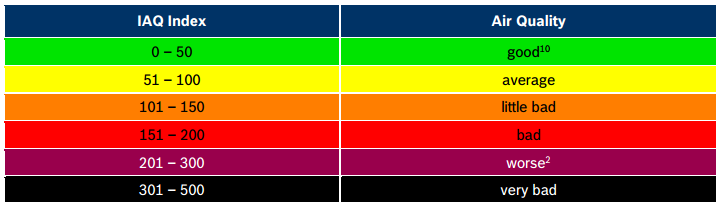
\includegraphics[width=0.8\textwidth]{Figures/Software/kw41z/bme680_iaq_indexes.PNG}
    \caption{Niveaux de l'indice IAQ}
    \label{fig-bme680_iaq_indexes}
\end{figure}

\begin{figure}[ht!]
    \centering
    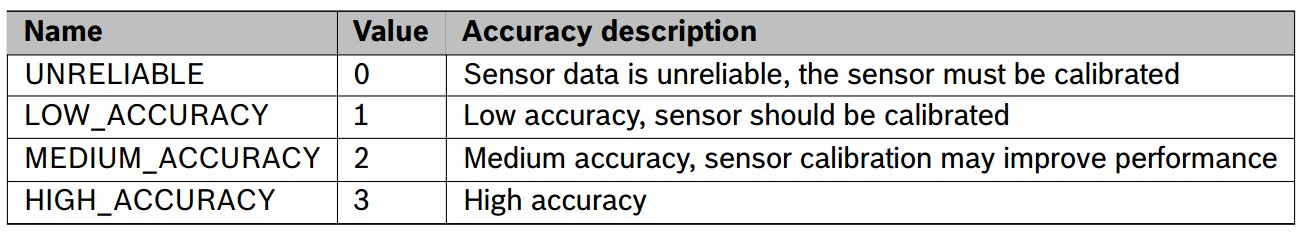
\includegraphics[width=0.8\textwidth]{Figures/Software/kw41z/iaq_accuracy.PNG}
    \caption{Niveaux de l'indice IAQ Accuracy}
    \label{fig-iaq_accuracy}
\end{figure}

Pour utiliser cette bibliothèque, le \textit{driver} BME680 doit être également utilisé et lié au projet. La qualité de l'air est mise à disposition à l'aide de l'indicateur \textit{Indoor Air Quality} (IAQ). Celle-ci est accompagnée d'un niveau de fiabilité nommé IAQ \textit{Accuracy}. L'IAQ est calculé à l'aide d'un algorithme propriétaire dont la valeur finale se situe entre 0 et 500. Les différents paliers de cet indice sont visibles sur la \cref{fig-bme680_iaq_indexes}. Selon le guide d'intégration de la bibliothèque BSEC \cite{BSEClib:online}, le périphérique nécessite 4 à 28 jours de calibration. Sur cette période, le composant doit être exposé 30min au milieu le moins pollué possible et 30min dans un milieu très pollué, afin de permettre une calibration plus correcte. La température et l'humidité sont également corrigées en fonction de l'environnement et la bibliothèque offre même la possibilité de placer un offset sur les valeurs pour prendre en compte l'échauffement des composants électroniques à proximité.



\subsubsection{Bibliothèques et \textit{drivers} développés}

Tous les fichiers présents sur la \cref{fig-board_paths} illustrant le répertoire \texttt{board} qui ne sont pas dans un sous répertoire ont été développés pour ce projet. Les sous-sections qui suivent ont pour but d'expliquer l'utilité des fichiers les plus importants. 


\subsubsubsection{\texttt{pin\_mux}}

\begin{figure}[ht!]
    \centering
    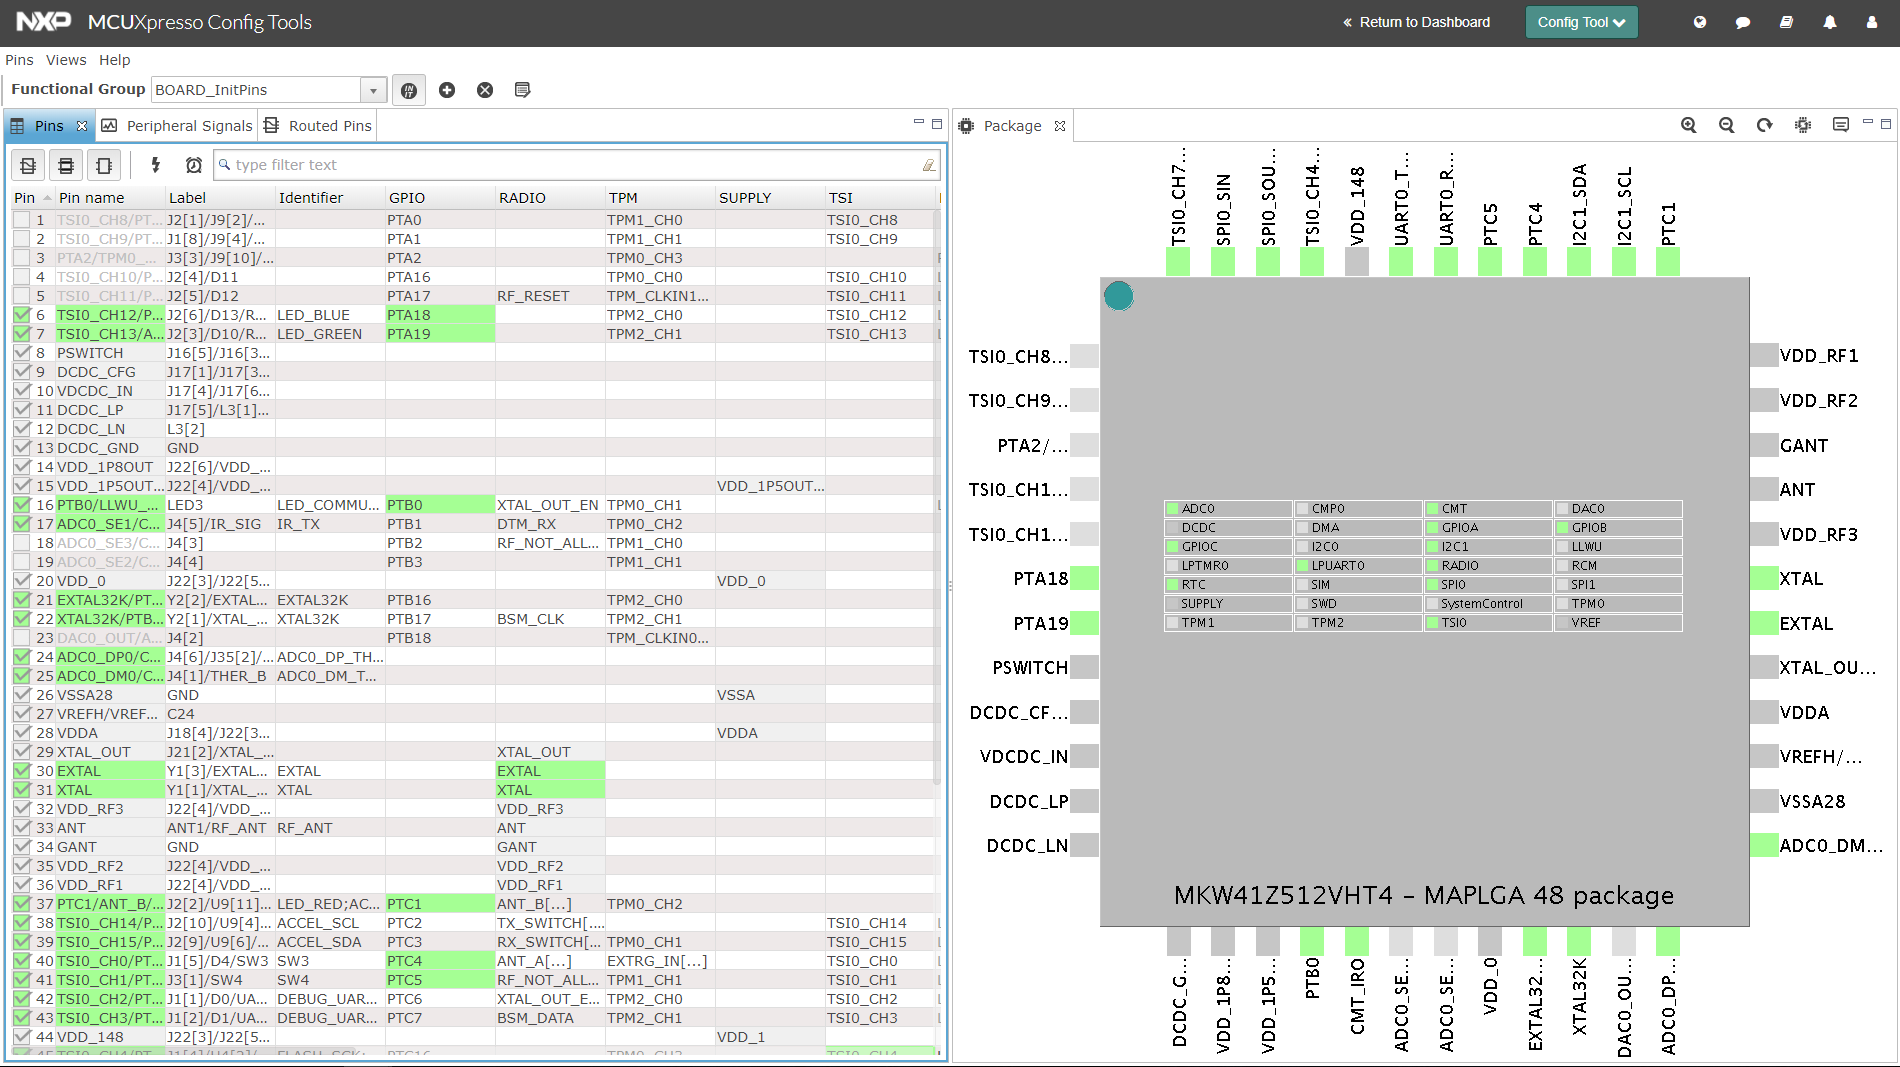
\includegraphics[width=1.0\textwidth]{Figures/Software/kw41z/mcuxpresso_pin_tools.PNG}
    \caption{Utilitaire de configuration du multiplexeur de pins des microcontrôleurs NXP}
    \label{fig-mcuxpresso_pin_tools}
\end{figure}


Le KW41Z est équipé d'un multiplexeur de pins, cela signifie que chaque pin peut avoir plusieurs rôles qui peuvent se modifier en cours d'exécutions. Pour aider les programmeurs, NXP propose dans le cadre de son SDK, un utilitaire nommé MCUXpresso Config Tools \footnote{\url{https://mcuxpresso.nxp.com/en/pins}}. Cet utilitaire est visible sur la \cref{fig-mcuxpresso_pin_tools}. Une fois les pins connectés sur l'utilitaire, il est possible d'exporter la configuration sous forme de fichier source afin d'être intégré au projet.


\subsubsubsection{\texttt{board}}

Une partie de ces deux fichiers est une reprise des divers exemples prodigués par NXP. Leur rôle est de fournir des accès génériques sans tenir compte du pinout appliqué au microcontrôleur. Par exemple, on peut y trouver une fonction nommée \path{BOARD_EnterLowPowerCb} offrant ainsi la possibilité de mettre le processeur en mode basse consommation. 


\subsubsubsection{\texttt{bme680 et bno055 support}}

Les drivers et bibliothèques du BME680 et BNO055 sont très bien fournis (cf. \cref{sec-softwaire_driver_bno} et \cref{sec-softwaire_driver_bme680}), mais il faut leur spécifier les interfaces matérielles qui communiquent avec le périphérique. Dans les deux cas, il s'agit d'un BUS I2C. Pour éviter tout problème de concurrence entre les tâches qui utilisent la même interface, le driver \path{fsl_i2c_freertos} a été utilisé dans ces deux bibliothèques. \\


La bibliothèque BSEC enregistre ponctuellement l'état de son algorithme d'apprentissage. Pour cela, il est nécessaire de fournir une fonction de sauvegarde en mémoire non volatile. Un secteur en flash a donc été réservé pour sauvegarder toutes les 2 heures l'état de la bibliothèque (fréquence de sauvegarde configurable). Une fonction de relecture de cette mémoire est également nécessaire, ainsi qu'une fonction pour la configuration utilisée (cf. le document \textit{Integration Guide
Bosch Software Environmental Cluster} (BSEC) \cite{BSEClib:online} pour toutes les configurations possibles). \\

Dans le cas du BME680, une fonction nommée \path{bme680_bsec_kw41z_iot_loop} s'occupe de réaliser l'acquisition en continu du capteur avec toute la gestion de la bibliothèque BSEC (capture, attente, sauvegarde de l'état de l'algorithme, etc.). L'utilisateur doit simplement fournir une fonction de \textit{callback} afin d'être notifié de la mesure d'un nouveau set de données, ainsi que divers paramètres concernant cette fréquence d'acquisition.

\subsubsubsection{\texttt{lorawan\_controller}}
\label{sec-softawre_kw41z_libs_lorawan_controller}

Le contrôleur LoRaWAN est l'un des éléments centraux de ce travail, c'est grâce à celui-ci qu'il est possible de configurer et de communiquer à travers un réseau LoRaWAN. Pour la communication avec le module LoRaWAN, les commandes AT sont envoyées à l'aide de la bibliothèque AT Commander (cf. \cref{sec-software_libs_atcommander}). Le contrôleur supervise également un espace mémoire en flash afin de stocker la configuration du module LoRaWAN dans but de se reconnecter au réseau lorsque le processeur est redémarré. Le contrôleur stocke en interne la configuration appliquée au module, ainsi que la nouvelle configuration que l'utilisateur souhaite appliquer à celui-ci. La structure \path{lorawanControllerConfiguration_t} a pour but de contenir toutes les informations de la configuration du module. À l'heure actuelle, l'AppKey est stockée sur le KW41Z, mais dans une version finale du système, celle-ci doit être stockée directement dans le module pour éviter que quelqu'un ne puisse intercepter la configuration lors de l'initialisation. Les attributs de cette structure sont listés ci-dessous :



\begin{tcolorbox}
  [top=-1mm, bottom=-3mm, left=0mm, right=0mm, enhanced,breakable,
  attach boxed title to top center={yshift=-3mm,yshifttext=-1mm},colback=LightGray,colframe=DarkGray,
  colbacktitle=DarkGray, fonttitle=\footnotesize\bfseries,boxed title style={size=small,colframe=DarkGray},
  title=\path{lorawan_controller.h} ]


\inputminted[firstline=30,lastline=54,bgcolor=LightGray,fontsize=\tiny,breaklines,linenos]{C}{SourceCode/lorawan_controller.h}
\end{tcolorbox}

Ces champs sont stockés sous forme de chaine de caractères. Cela est dû au fait que la communication avec le module LoRaWAN est basée sur des commandes AT, et donc les paramètres de ces commandes sont tous des \textit{strings}. Afin d'économiser du temps CPU dans la conversion des données lors de l'envoi de chaque commande au module, il a été décidé de garder ce format tout au long du processus, au risque d'occuper plus d'espace mémoire. Un CRC codé sur 16bits a été ajouté à la configuration, à la suite de plusieurs problèmes liés à l'écriture et à la lecture de la mémoire flash. Ces problèmes ont été résolus, mais ce CRC a été maintenu puisque si la carte s'éteint lors de l'écriture en flash, les données peuvent toujours être corrompues. Si le CRC est erroné lors de la lecture d'une configuration, la configuration par défaut est appliquée. 

\begin{figure}[ht!]
    \centering
    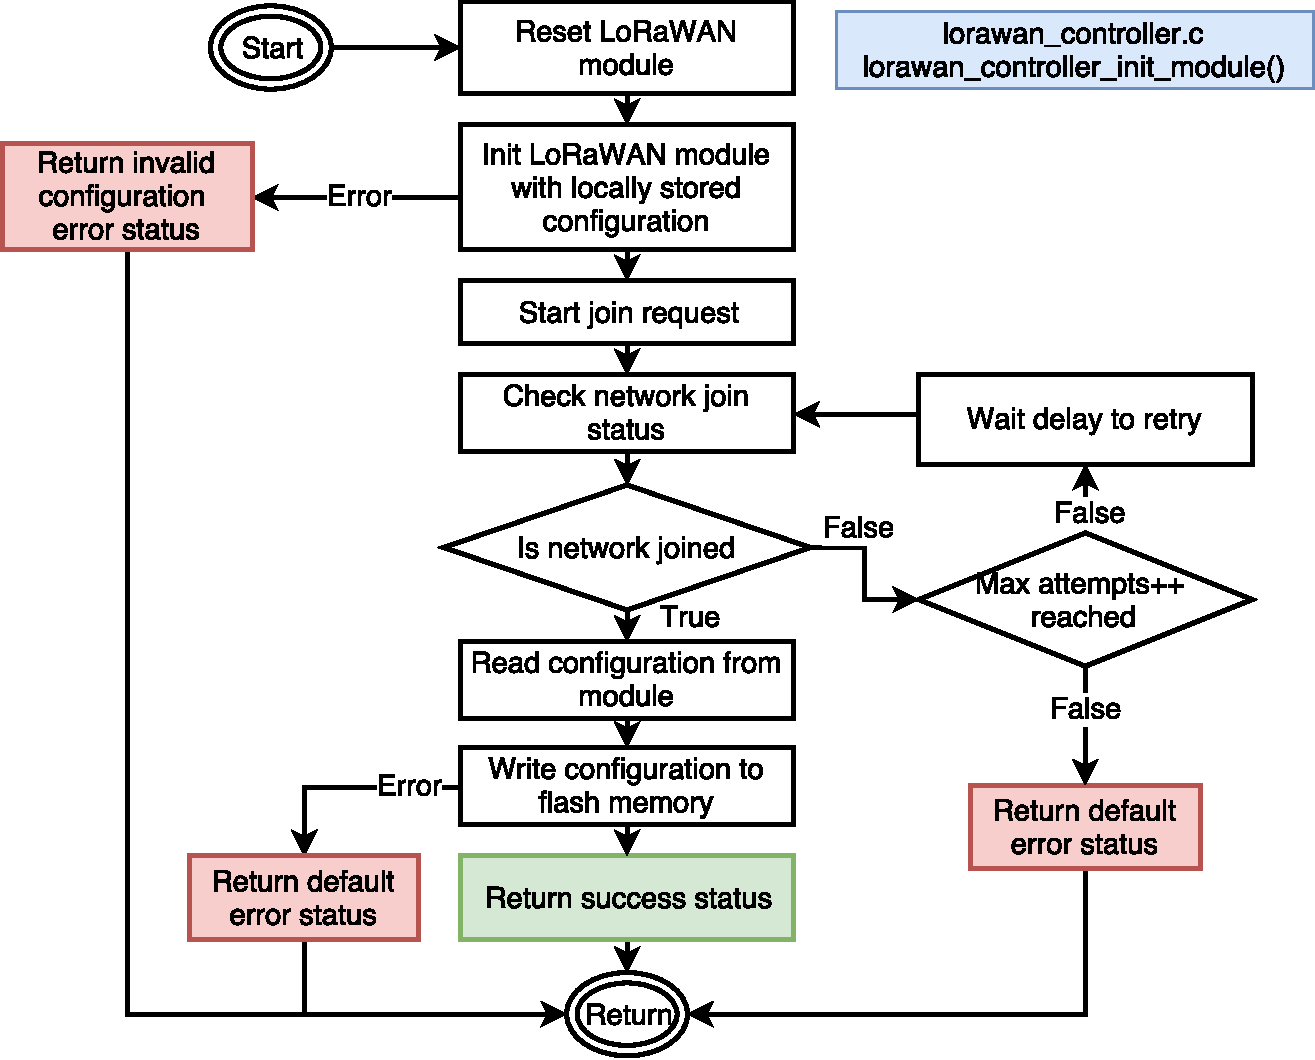
\includegraphics[width=0.8\textwidth]{Figures/Software/diagram_lorawan_init_module.pdf}
    \caption{Diagramme de la fonction d'initialisation du module LoRaWAN}
    \label{fig-diagram_lorawan_init_module}
\end{figure}

L'une des étapes les plus importantes du module est son initialisation. L'initialisation s'effectue à l'aide de la fonction \path{lorawan_controller_init_module}. Un diagramme représentant l'algorithme utilisé est visible sur la \cref{fig-diagram_lorawan_init_module}. En observant ce diagramme, on constate que la configuration du module est sauvegardée uniquement lorsque le réseau a pu être correctement rejoint à l'aide d'un \textit{Join Request}. Tant que la demande de \textit{join} n'est pas confirmée, le contrôleur est bloqué. Un temps d'attente maximum est configurable dans le contrôleur en spécifiant le nombre de vérifications du statut de \textit{join} avec le temps d'attente entre chacune de ces vérifications.

\subsubsubsection{\texttt{neo-m8}}
 \label{sec-software_libs_neom8}

Ces fichiers contiennent toutes les fonctions pour récupérer les données provenant du NEO M8 avec le support de l'interruption du signal \texttt{timepulse} pour démarrer l'acquisition. Une fois les données récupérées, il est possible de spécifier une fonction de \textit{callback} à l'aide d'un pointeur pour informer l'application de la réception de nouvelles mesures. Ces mesures sont ensuite accessibles par l'application en utilisant le parseur minmea (cf. \cref{sec-software_libs_minmea}). Cette bibliothèque est principalement utilisée par la tâche GPS présentée en \cref{sec-software_kw41z_algo_gps}.\\


Le NEO M8 supporte le protocole propriétaire UBX afin de communiquer avec le GPS pour le configurer. Cette configuration n'a pas été mise en place à l'heure actuelle, principalement par manque de temps. Toutefois, si l'on souhaite avoir un système base consommation, le support de ce protocole doit être fait. Plusieurs bibliothèques sont disponibles pour le protocole UBX\footnote{\url{https://github.com/arobenko/ublox}}, cependant peu d'entre elles sont orientées systèmes embarqués avec de faibles ressources. Le protocole UBX est très conséquent et nécessite beaucoup de place en mémoire. Par défaut le GPS envoie des trames GPS NMEA avec un intervalle de 1 seconde et sans la possibilité d'être mis en mode \textit{sleep}. Ces paramètres sont uniquement modifiables à l'aide du protocole UBX.

\subsubsubsection{\texttt{string\_utils}}

Dans ce projet, il est souvent nécessaire de faire des conversions entre plusieurs formats de données. Le type de conversion le plus utilisé est le tableau de \textit{bytes} en \textit{string} et vice versa. Des fonctions ont donc été développées et placées à l'intérieur de ces fichiers.


% ---------------------------------------------------------------------------------------------%
\FloatBarrier
\subsection{Architecture des tâches}
\label{sec-smartcanton_tasks_overview}
% ---------------------------------------------------------------------------------------------%

Dans ce projet, il a été décidé de faire en sorte que la communication entre les tâches soit le plus uniforme possible. L'idée est de permettre à l'utilisateur de désactiver simplement une tâche, s'il le souhaite. 

\begin{figure}[ht!]
    \centering
    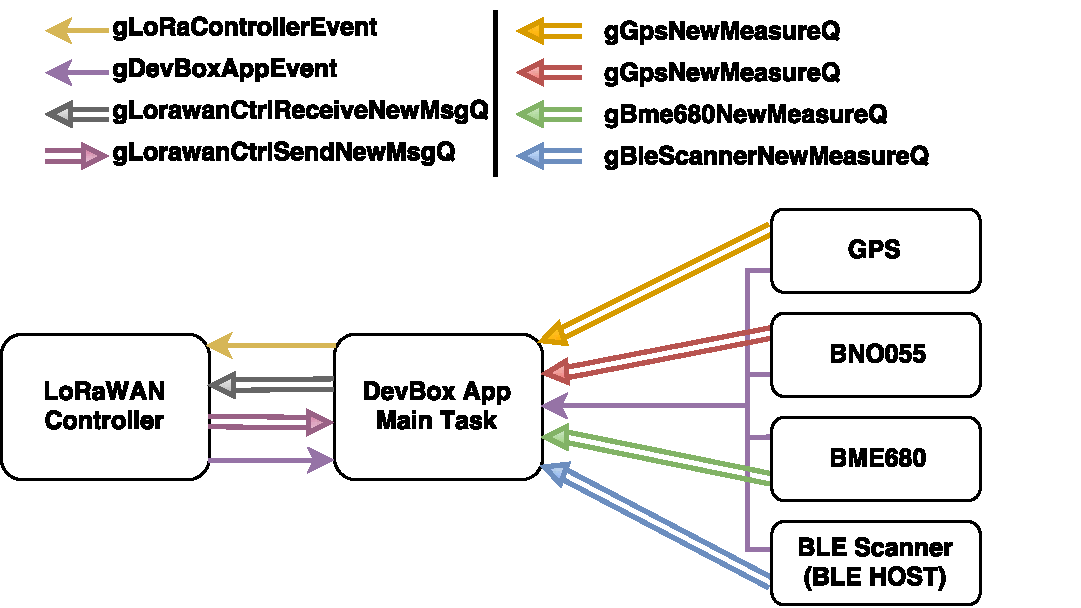
\includegraphics[width=1.0\textwidth]{Figures/Software/smartcanton_tasks_overview.pdf}
    \caption{Vue générale des communications entre les tâches}
    \label{fig-smartcanton_tasks_overview}
\end{figure}

À l'aide de la \cref{fig-smartcanton_tasks_overview}, il est possible de voir les différentes tâches implémentées ainsi que les mécanismes de communication mis en place. Chaque tâche produisant des données de ses capteurs dispose d'une \textit{queue} (file) dans laquelle elle va alimenter les données des captures. Une fois ces données dans cette file, une notification est envoyée à la tâche principale à l'aide d'un événement. La tâche principale attend en permanence sur cet événement pour agir en conséquence. Dans les RTOS, il est possible d'attendre sur l'arrivée de données provenant des \textit{queues}, mais il n'est pas envisageable d'écouter plusieurs flux en même temps, du moins, en utilisant l'OSA. 
Toutes les tâches utilisent des attentes sur des signaux, ce qui permet d'économiser le temps du processeur contrairement aux attentes actives (scrutations). S'agissant là d'un système embarqué, la consommation liée à ces ressources est un facteur important.


% ---------------------------------------------------------------------------------------------%
\FloatBarrier
\subsection{Algorithmes des tâches}
% ---------------------------------------------------------------------------------------------%
Le but de cette section est de présenter les différentes étapes qui se déroulent dans les différentes tâches d'acquisition des données. Le but n'est pas d'entrer dans les détails, mais d'avoir un aperçu global du \textit{workflow} implémenté dans chaque tâche.


% ---------------------------------------------------------------------------------------------%
\FloatBarrier
\subsubsection{DevBox Main}

La \cref{fig-smartcanton_tasks_overview} explique la synchronisation à l'aide de l'envoi d'événements avec la tâche principale. Le nom de l'événement est \texttt{gDevBoxAppEvent} et peut transmettre les types d'événements suivants : 
\begin{tcolorbox}
  [top=-1mm, bottom=-3mm, left=0mm, right=0mm, enhanced,breakable,
  attach boxed title to top center={yshift=-3mm,yshifttext=-1mm},colback=LightGray,colframe=DarkGray,
  colbacktitle=DarkGray, fonttitle=\footnotesize\bfseries,boxed title style={size=small,colframe=DarkGray},
  title=\texttt{dev\_box\_app\_task.h} ]
\inputminted[firstline=63,lastline=93,bgcolor=LightGray,fontsize=\tiny,breaklines,linenos]{C}{SourceCode/dev_box_app_task.h}
\end{tcolorbox}

La tâche DevBox Main est la tâche principale de toute l'application. Elle a comme rôle de connecter les données des capteurs avec les différentes interfaces de communications disponibles. Voici la liste des opérations qui lui incombent : 

\begin{enumerate}
    \item Son rôle principal est de récupérer les données des divers capteurs présents sur la carte. Ces données sont ensuite stockées en local dans un historique temporaire.
    
    \item De manière générale, tous les services Bluetooth sont actualisés par cette tâche afin de garder une certaine structure dans le code et ainsi éviter des problèmes de fragmentations. Par exemple, lorsqu'un réseau LoRaWAN est rejoint, le contrôleur informe la tâche principale que les services doivent être mis à jours. De même pour les capteurs, les mesures reçues des tâches adjacentes sont également mises à jour dans les services Bluetooth Low Energy correspondants (cf. \cref{sec-software_ble_services}).
    
    \item Périodiquement, la tâche envoie des données sur le réseau LoRaWAN. L'envoi de nouvelles données s'effectue à l'aide d'un \textit{timer} qui définit l'intervalle entre chaque paquet LoRaWAN. Le paquet contient toujours les dernières données qui ont été sauvegardées localement. Cet intervalle est à ce jour uniquement configurable lors de la réception d'un paquet \textit{downlink} depuis le réseau.
    
    \item Les paquets \textit{downlink} LoRaWAN sont transmis à la tâche afin que l'application agisse en conséquence.
\end{enumerate}



En fonction du type d'événements reçus, une action est réalisée. En attendant l'événement, la tâche ne consomme pas de ressources. Une représentation simplifiée de l'algorithme appliqué dans la tâche est visible sur le diagramme \cref{fig-diagram_main_task}. 

\begin{figure}[ht!]
    \centering
    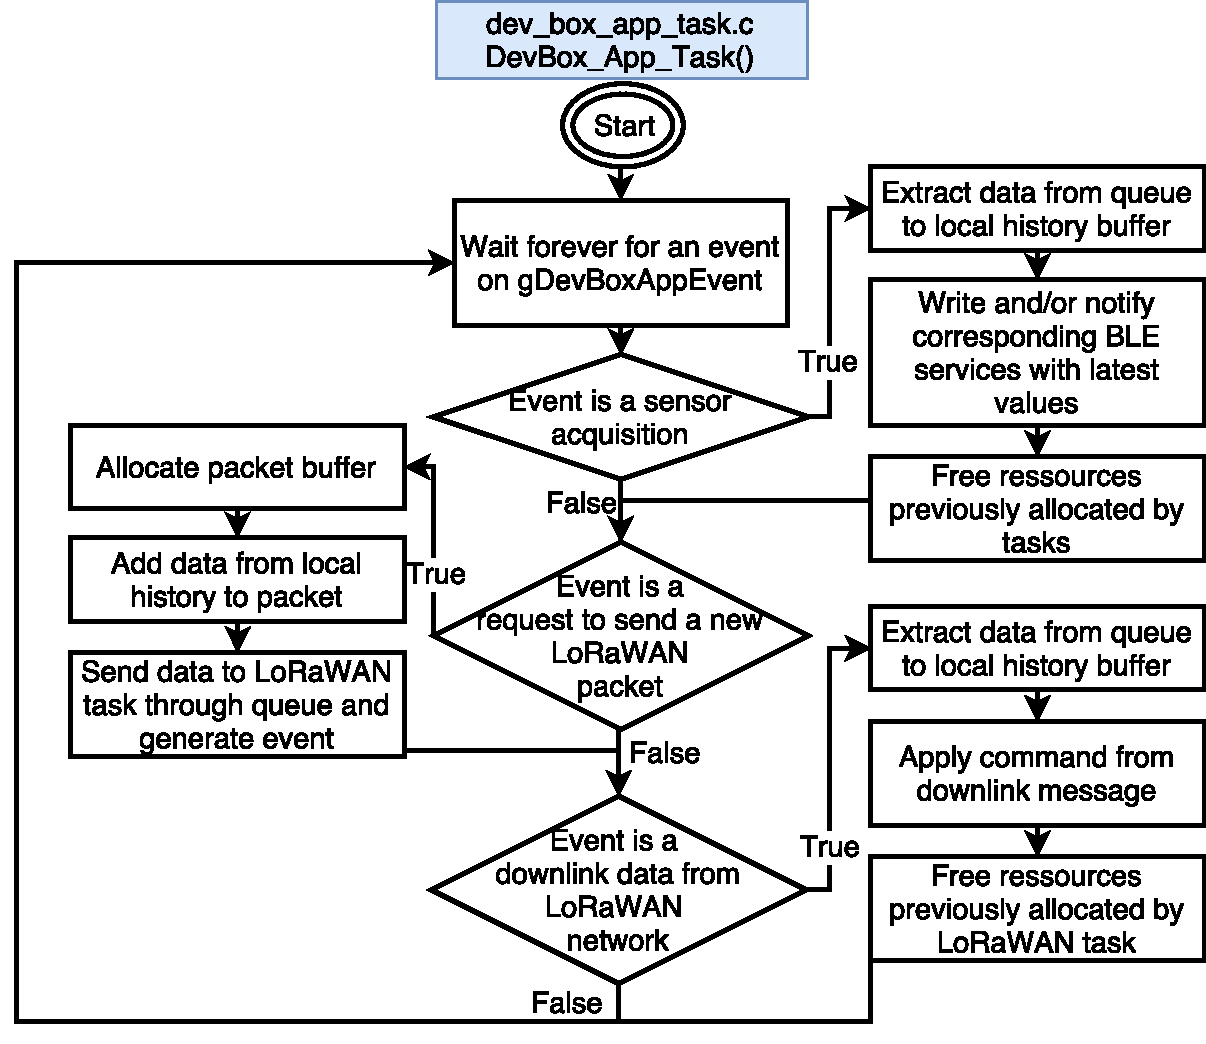
\includegraphics[width=0.8\textwidth]{Figures/Software/diagram_main_task.pdf}
    \caption{Diagramme de fonctionnement de la tâche principale lors de la gestion des événements}
    \label{fig-diagram_main_task}
\end{figure}

% ---------------------------------------------------------------------------------------------%
\FloatBarrier
\subsubsection{GPS Neo M8}
\label{sec-software_kw41z_algo_gps}


\begin{figure}[ht!]
    \centering
    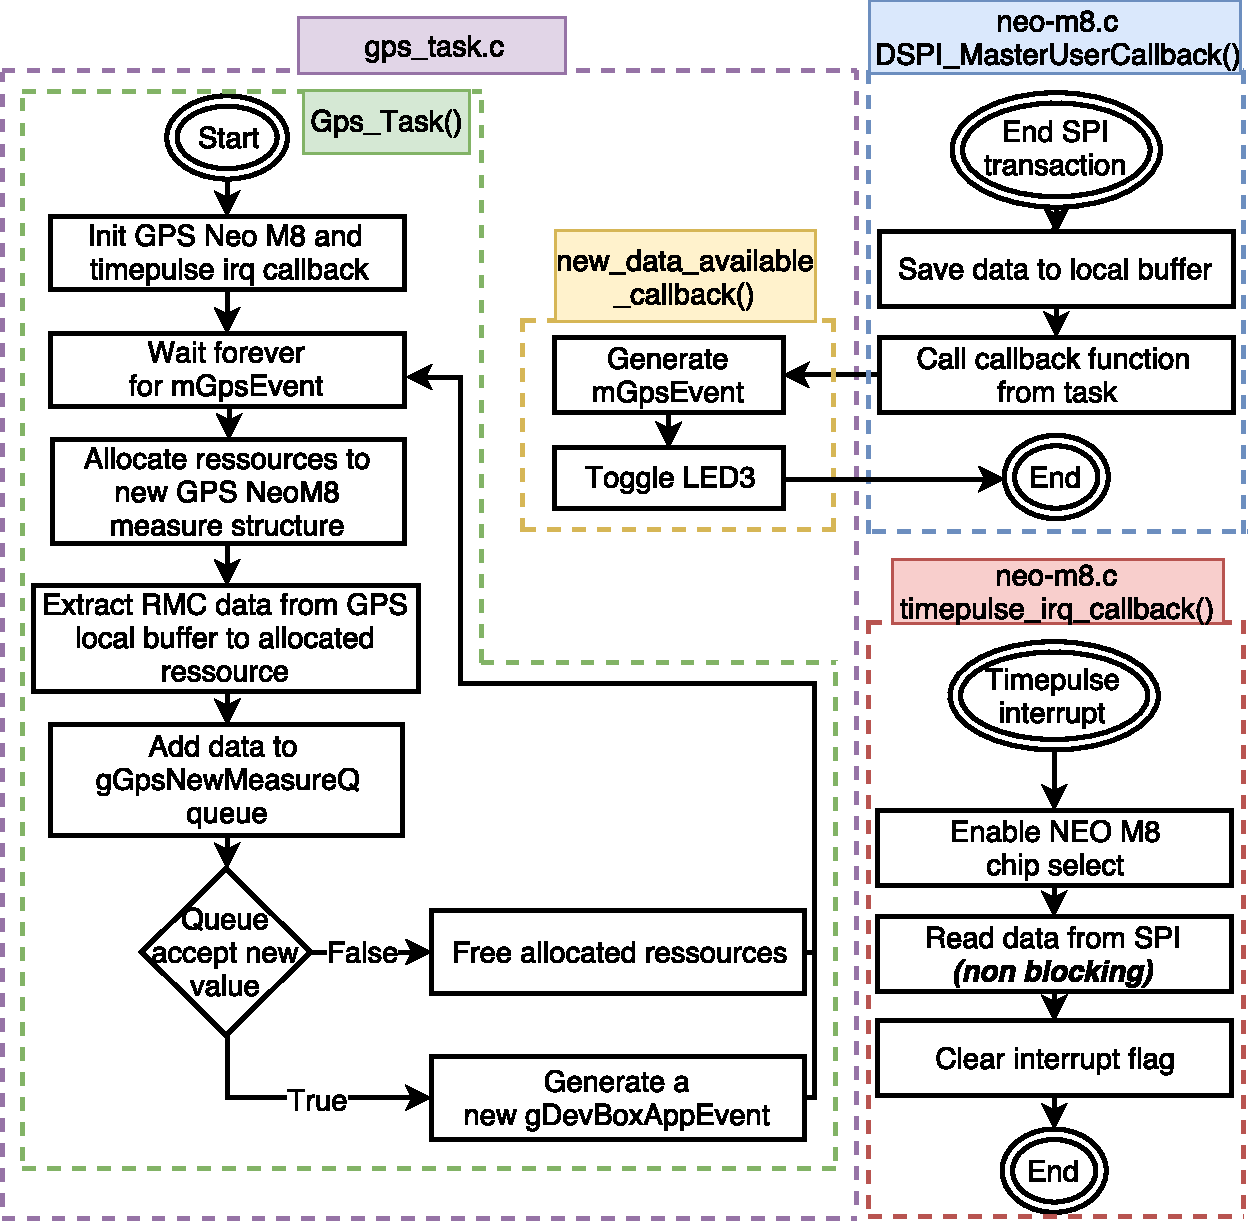
\includegraphics[width=0.8\textwidth]{Figures/Software/diagram_gps_neo.pdf}
    \caption{Diagramme de fonctionnement de la tâche GPS}
    \label{fig-diagram_gps_neo}
\end{figure}

Le GPS génère périodiquement des trames NMEA qui doivent être lues à l'aide de l'interface SPI du KW41Z. Toute cette acquisition est gérée par la bibliothèque nommée neo-m8 (cf. \cref{sec-software_libs_neom8}). À l'heure actuelle, la LED numéro 3 de la carte change d'état pour indiquer que la synchronisation avec le GPS est correcte et qu'au minimum la synchronisation temporelle est possible (\textit{timepulse}). La \cref{fig-diagram_gps_neo} illustre les différentes étapes de l'acquisition et l'envoi des données à l'aide du processus d'échange expliqué précédemment pour la tâche GPS.


% ---------------------------------------------------------------------------------------------%
\FloatBarrier
\subsubsection{BNO055}

\begin{figure}[ht!]
    \centering
    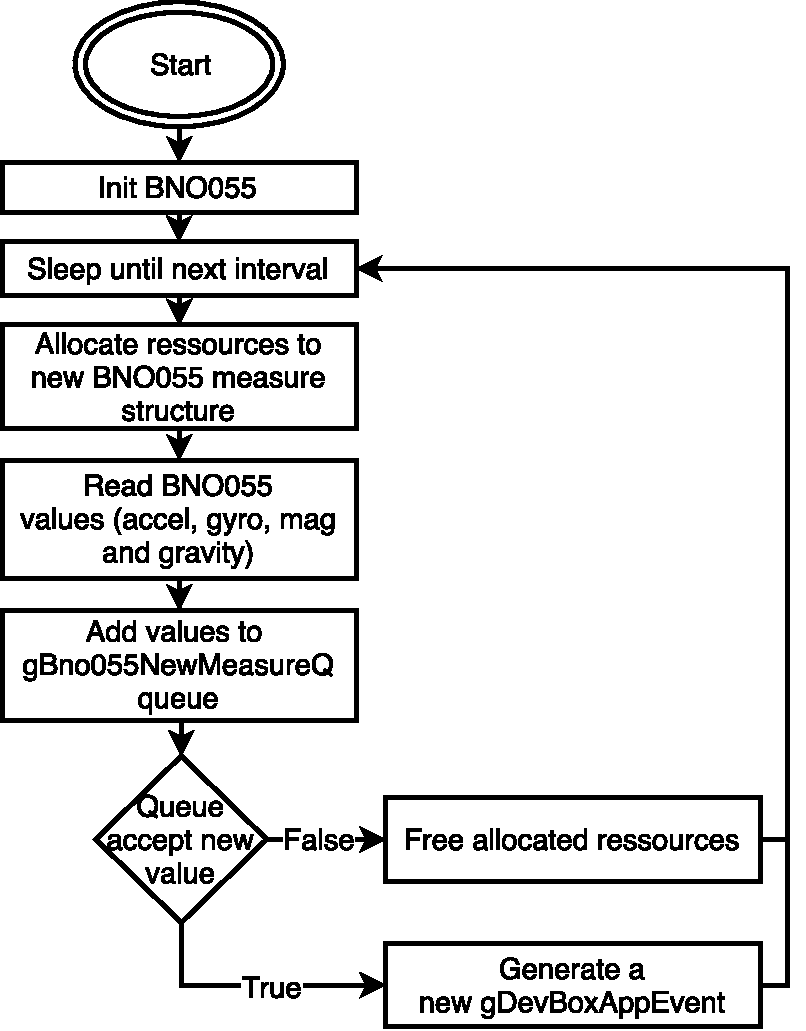
\includegraphics[width=0.50\textwidth]{Figures/Software/diagram_bno055.pdf}
    \caption{Diagramme de fonctionnement de la tâche BNO055}
    \label{fig-diagram_bno055}
\end{figure}

La \cref{fig-diagram_gps_neo} illustre les différentes étapes pour l'acquisition et l'envoi des données pour la tâche du BNO055. L'intervalle entre les mesures est configurable à l'aide d'une fonction appelée lors de l'écriture d'une caractéristique Bluetooth correspondante.

L'implémentation actuelle n'est pas adéquate si l'utilisateur souhaite utiliser une fréquence d'échantillonnage fixe et automatisée par le périphérique. Dans ce cas-là, il faut configurer le BNO055 afin qu'il génère une interruption lorsqu'un \textit{sample} est prêt à être récolté. La gestion de l'interruption a été gérée au niveau de la tâche, il manque juste la configuration du BNO055.




% ---------------------------------------------------------------------------------------------%
\FloatBarrier
\subsubsection{BME680}

\begin{figure}[ht!]
    \centering
    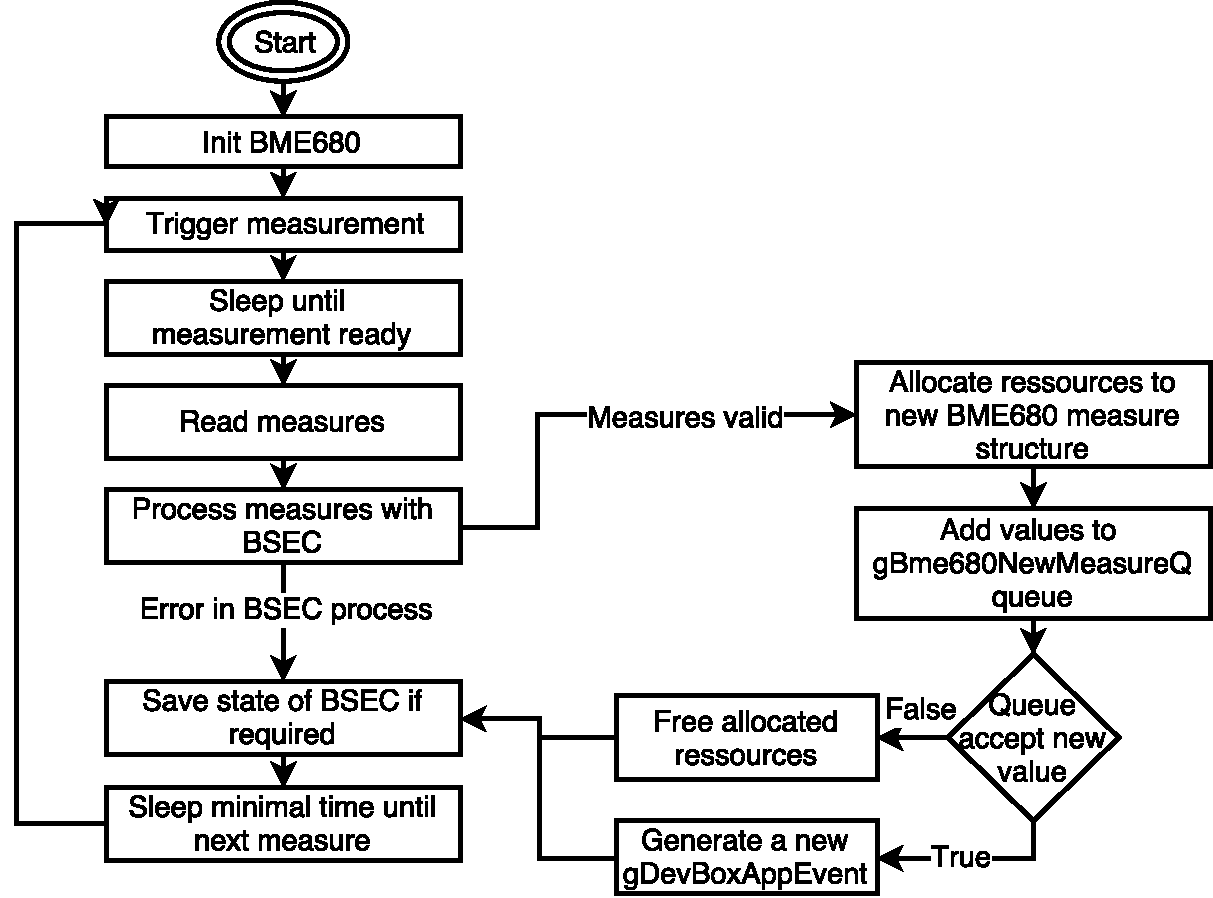
\includegraphics[width=0.7\textwidth]{Figures/Software/diagram_bme680.pdf}
    \caption{Diagramme de fonctionnement de la tâche BME680}
    \label{fig-diagram_bme680}
\end{figure}

La bibliothèque BSEC s'occupe d'une grande partie de l'acquisition et du traitement des données provenant du capteur, comme expliqué en \cref{sec-software_bme680_bsec}. Il reste donc peu d'éléments à être gérés par la tâche. La \cref{fig-diagram_bme680} illustre les différentes étapes pour l'acquisition et l'envoi des données sous forme d'un diagramme.



% ---------------------------------------------------------------------------------------------%
\FloatBarrier
\subsubsection{Scanneur Bluetooth Low Energy}

\begin{figure}[ht!]
    \centering
    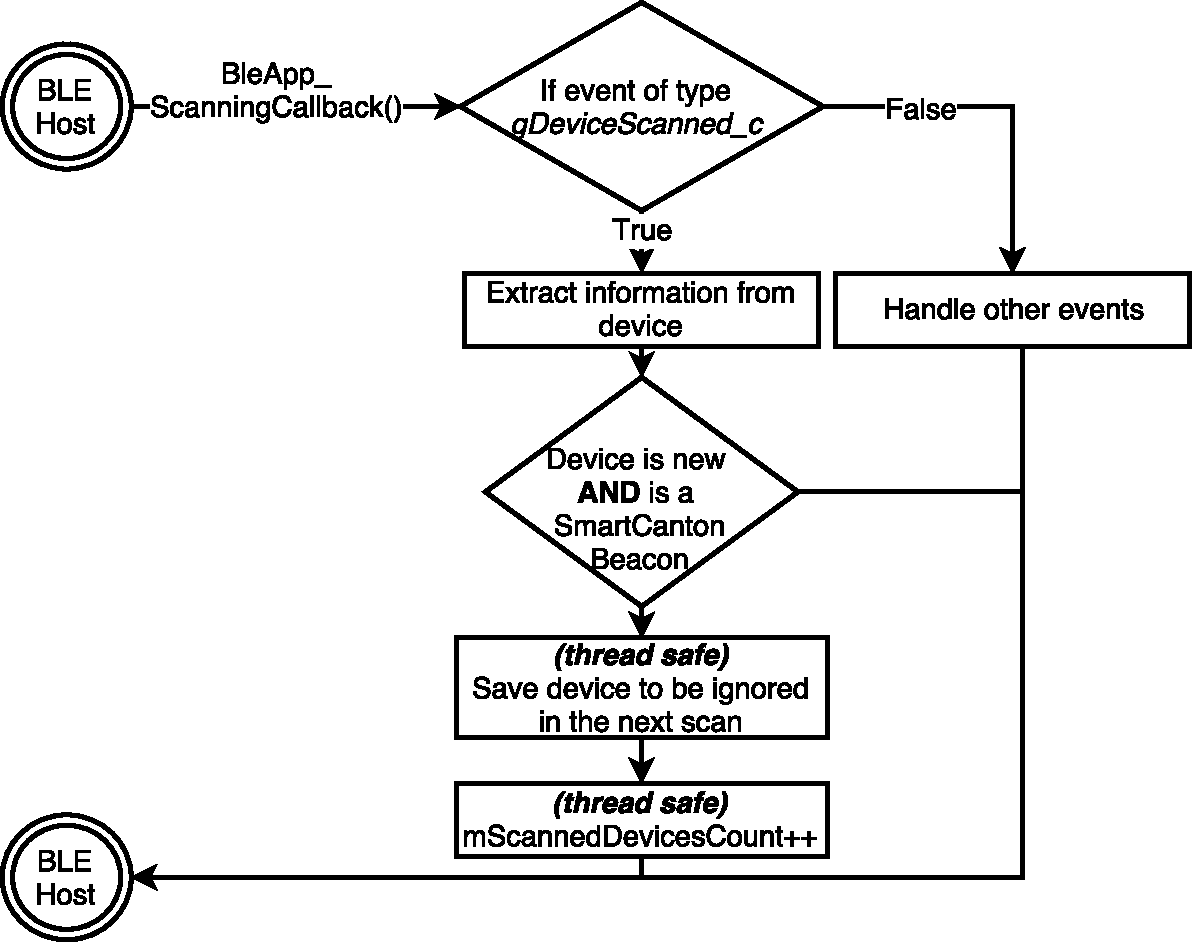
\includegraphics[width=0.7\textwidth]{Figures/Software/diagram_blescanner_parsing.pdf}
    \caption{Diagramme de fonctionnement de la tâche scanneur Bluetooth lors de la sauvegarde des nouveaux périphériques}
    \label{fig-diagram_blescanner_parsing}
\end{figure}

\begin{figure}[ht!]
    \centering
    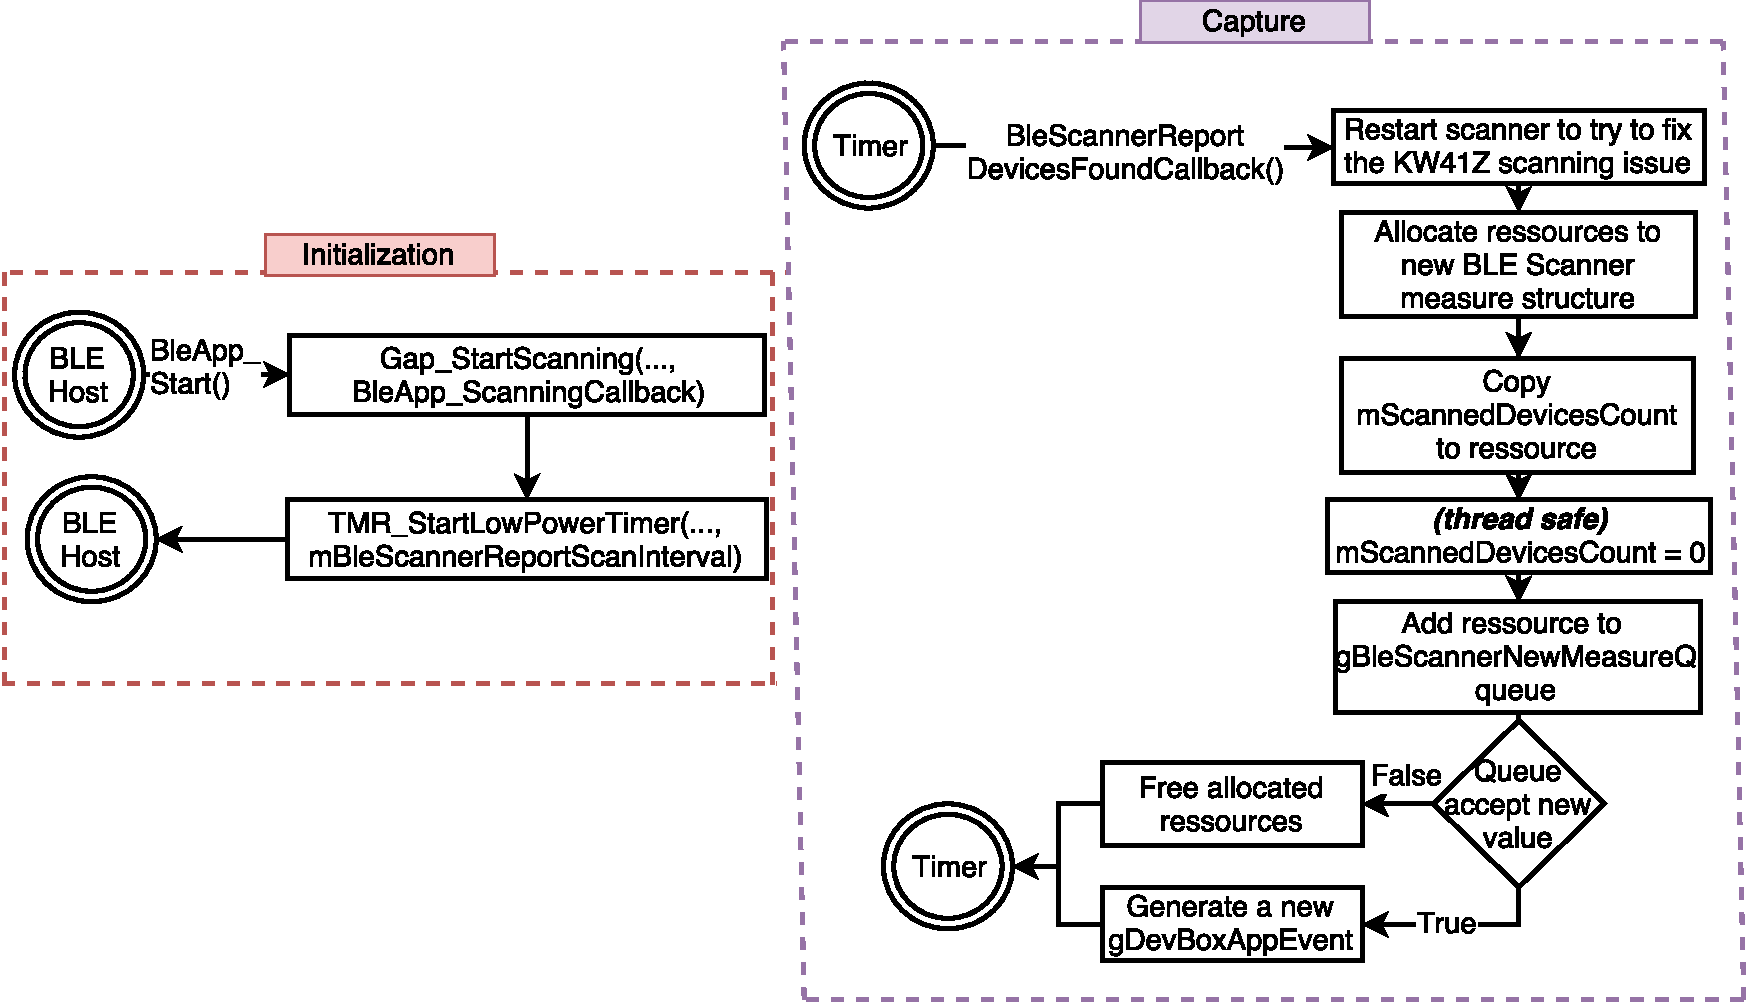
\includegraphics[width=1.0\textwidth]{Figures/Software/diagram_blescanner_init_acsquisition.pdf}
    \caption{Diagramme de fonctionnement de la tâche de scanneur Bluetooth lors de son initialisation et de la capture des données}
    \label{fig-diagram_blescanner_init_acsquisition}
\end{figure}

Le scanneur Bluetooth n'a pas de tâche propre à lui seul. Il dépend de la tâche \textit{Host} de la \textit{stack} Bluetooth. C'est celle-ci qui appelle une fonction \textit{callback} lorsque de nouveaux périphériques scannés sont disponibles. Il y a donc deux éléments en parallèle. Premièrement, le scanneur qui est directement implémenté par l'hôte et dont le code du \textit{callback} d'un nouveau périphérique BLE est décrit . En deuxième lieu, il y a un \textit{timer} qui récupère le nombre de périphériques qui ont été scannés et qui transfère cette valeur à la tâche principale du système (cf. \cref{fig-diagram_blescanner_init_acsquisition}). Le lancement du scan s'effectue au démarrage de l'application avec l'appel de la fonction \path{BleApp_Start}, démontré en \cref{fig-diagram_blescanner_init_acsquisition}. 






% ---------------------------------------------------------------------------------------------%
\FloatBarrier
\subsubsection{LoRaWAN \textit{Controller}}


La tâche LoRaWAN est le n\oe ud central pour communiquer avec le contrôleur LoRaWAN. Son interface est également basée sur des événements présentés sur la \cref{fig-smartcanton_tasks_overview} avec l'utilisateur. C'est elle qui régit l'état lié au contrôleur LoRaWAN avec l'envoi des différentes commandes pour rejoindre et transmettre des données sur le réseau. Tous les messages sont stockés dans une \textit{queue} pour éviter qu'il ne soit perdu si un message est déjà en cours d'envoi, ou que le \textit{duty cycle} maximum a été atteint. Cette tâche notifie également la tâche principale quand le réseau a pu être rejoint correctement afin d'effectuer les actions nécessaires à l'acquisition des capteurs. Le fonctionnement de l'algorithme de cette tâche est visible sur la \cref{fig-diagram_lorawan_controller}.

\begin{figure}[ht!]
    \centering
    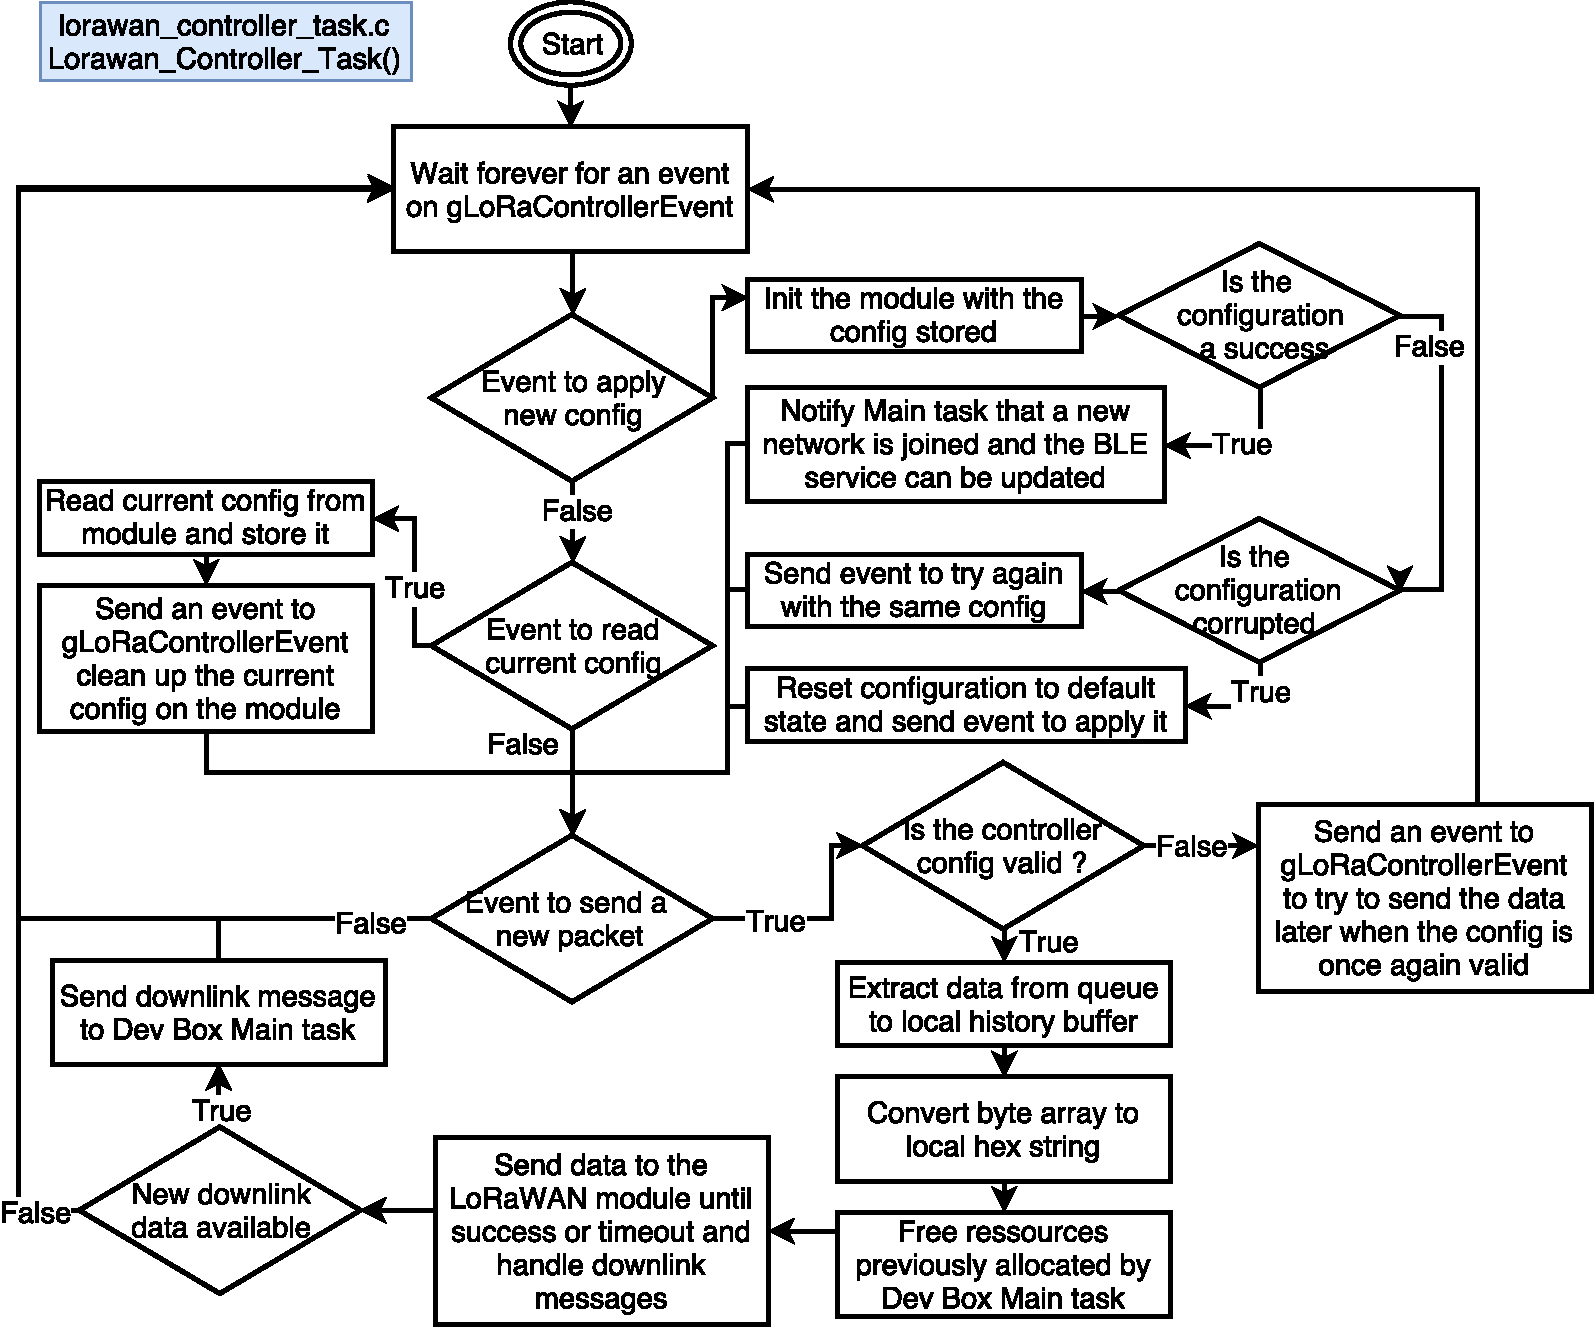
\includegraphics[width=1.0\textwidth]{Figures/Software/diagram_lorawan_controller.pdf}
    \caption{Diagramme de fonctionnement de la tâche \texttt{LoRaWAN Controller} lors de la gestion des événements}
    \label{fig-diagram_lorawan_controller}
\end{figure}






\FloatBarrier
% ---------------------------------------------------------------------------------------------%
\subsection{KW41Z \textit{stack} Bluetooth}
% ---------------------------------------------------------------------------------------------%
La \textit{stack} Bluetooth du KW41Z suit le modèle présenté en \cref{sec-protocols_ble}. Celle-ci n'est pas open source, ce qui peut parfois complique le développement quand une erreur se produit à l'intérieur de celle-ci. L'utilisateur a très peu de contrôle sur l'interface contrôleur. Les tâches qui gèrent le contrôleur et l'hôte ne sont pas directement modifiables par l'utilisateur, contrairement à la couche application qui est entièrement open source et dont plusieurs exemples sont proposés. \\

Le SDK fournit par NXP est personnalisable par l'utilisateur à l'aide d'un portail en ligne sur le site de NXP, nommé \textit{MCUXpresso SDK Builder}, et visible sur la \cref{fig-mcuxpresso_sdk_platform}. L'utilisateur peut ainsi choisir quel microcontrôleur utiliser et personnaliser les différentes bibliothèques qui sont ajoutées au SDK. Ce SDK est ensuite compilé sur la plateforme en ligne et dans un second temps, un e-mail est ensuite envoyé quand la compilation est achevée. Une archive doit pour la suite être téléchargée et ajoutée à l'IDE MCUXpresso. Divers exemples de projets sont disponibles pour des cartes de développement impliquant le microcontrôleur choisi et ainsi accélérer le développement pour le programmeur. Dans le cadre de ce travail, le projet de base utilisé est celui nommé \texttt{\path{frdmkw41z_wireless_examples_bluetooth_heart_rate_sensor_freertos}} basé sur la carte de développement FRDMKW41Z présentée en \cref{sec-hardware_kw41z}.

\begin{figure}[ht!]
    \centering
    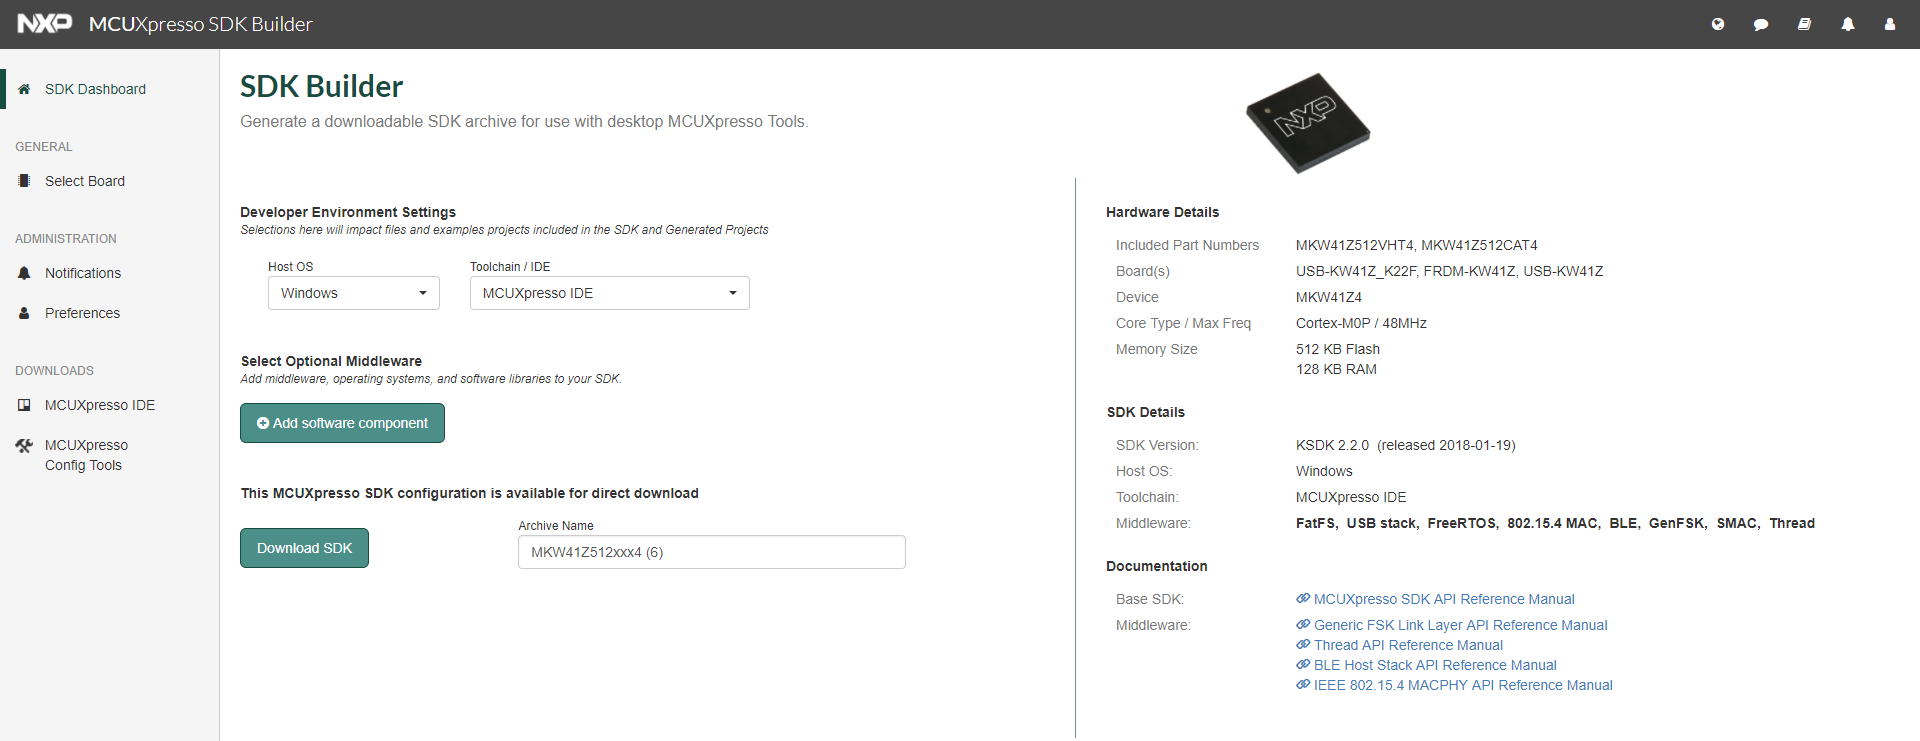
\includegraphics[width=1.0\textwidth]{Figures/Software/kw41z/mcuxpresso_sdk_platform.PNG}
    \caption{MCUXpresso SDK Builder interface}
    \label{fig-mcuxpresso_sdk_platform}
\end{figure}


\FloatBarrier
% ---------------------------------------------------------------------------------------------%
\subsection{Services Bluetooth}
\label{sec-BLEAllServices}
% ---------------------------------------------------------------------------------------------%


La déclaration des services Bluetooth s'effectue à l'aide de deux fichiers nommés \texttt{\path{gatt_uuid128.h}} et \texttt{\path{gatt_db.h}}. Le premier contient uniquement les UUID des différents attributs des services Bluetooth. Ces UUIDs sont créés à l'aide d'une macro nommée \texttt{UUID128} ayant comme paramètre une variable qui contiendra le UUID, suivi d'un tableau de bytes de 16 emplacements. Le deuxième fichier est celui qui permet de créer toute la structure des services Bluetooth, avec la spécification des services, caractéristiques et descripteurs nécessaires. \\


Une partie de ces fichiers peut être générée à l'aide d'un \textit{plug-in} de Freescale pour le logiciel Bluetooth Developper Studio\footnote{\url{https://www.bluetooth.com/develop-with-bluetooth/developer-resources-tools/developer-kits/bluetooth-developer-plugins}} (BDS). Toutefois, ce \textit{plug-in} n'a pas été mis à jour depuis plusieurs versions du SDK. Celui-ci remonte à la version 1.3, alors que la version actuellement supportée est la version 2.2. BDS est développé par le Bluetooth \textit{Special Interest Group} (SIG) et a pour but d'accélérer l'utilisation de profils standards (ex. \textit{Hearth Rate Sensor} HRS)) ou des profils personnalisés. Le logiciel est téléchargeable gratuitement à l'adresse suivante :

\begin{center}
    \url{https://www.bluetooth.com/download-developer-studio}
\end{center}

\begin{figure}[ht!]
    \centering
    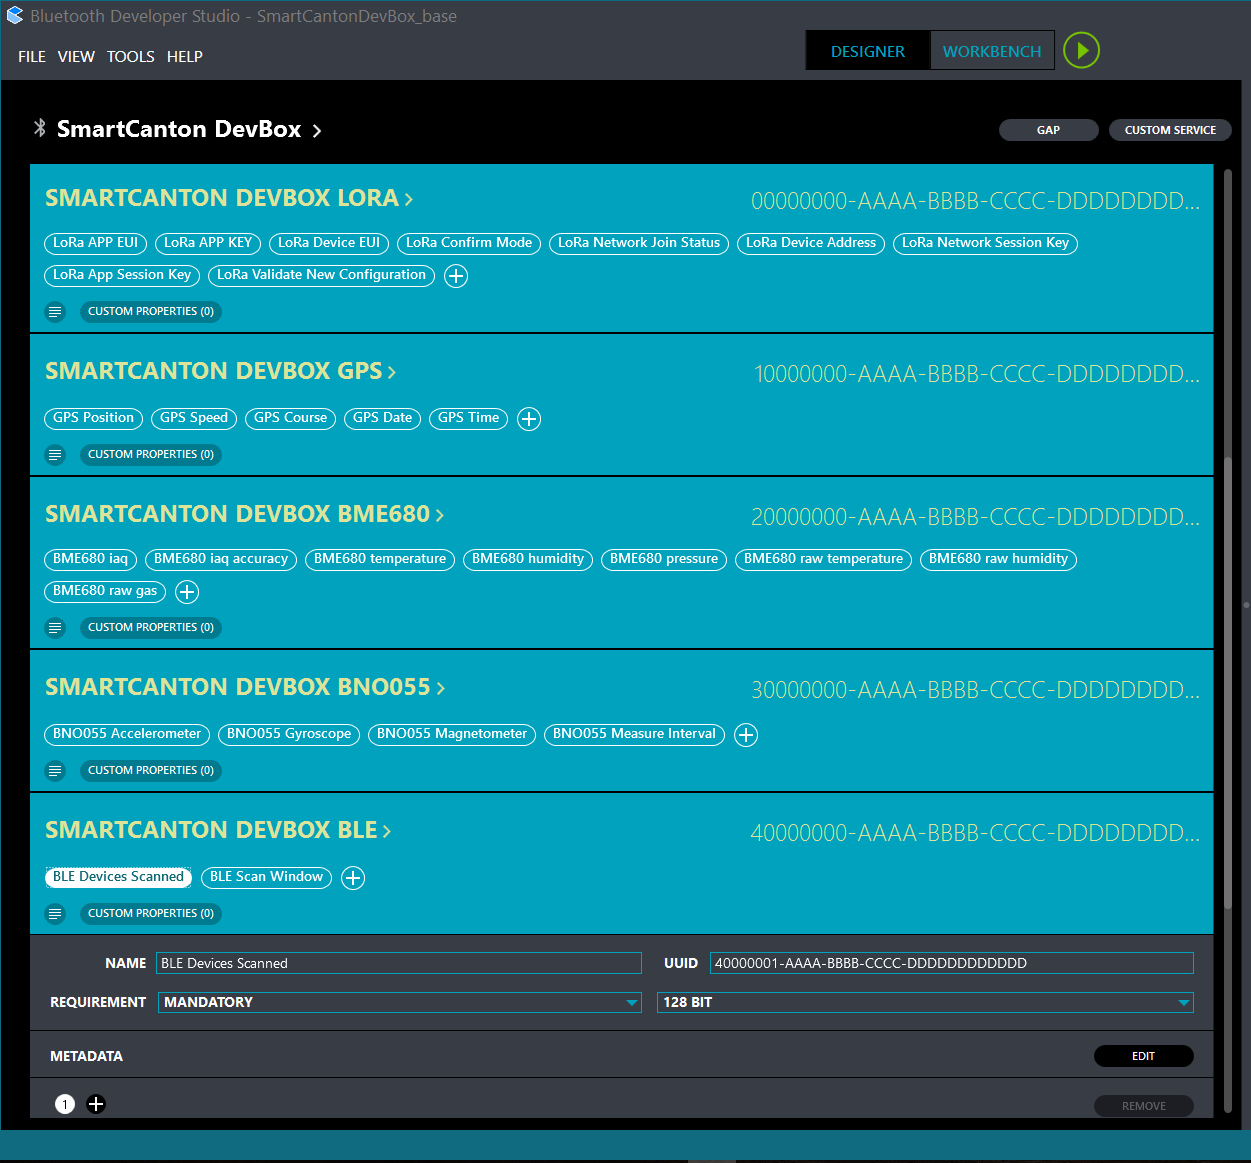
\includegraphics[width=1.0\textwidth]{Figures/Software/kw41z/bds_interface_smartcanton.png}
    \caption{Bluetooth Developer Studio avec les services BLE du projet SmartCanton DevBox}
    \label{fig-bds_interface_smartcanton}
\end{figure}

Dans ce projet, tous les services ont été créés à l'aide de cet outil. Si un jour le microcontrôleur utilisé n'est plus le KW41Z, mais un autre, par exemple un NRF52, il est très facile d'exporter les profils personnalisés. Le projet de BDS est disponible dans le dépôt GitHub, dans le répertoire \path{dev/BluetoothDeveloperStudio}. L'interface de ce projet dans BDS est visible sur la \cref{fig-bds_interface_smartcanton}. \\


En section \cref{sec-protocols_BLE_services}, les descripteurs de type CCCD ont été évoqués, de même que la liste des différents descripteurs attribuables aux caractéristiques. Il existe des descripteurs de type \textit{Characteristic User Description Descriptor} (CUDD), qui sont entièrement personnalisables par l'utilisateur. En effet, comme on peut le voir sur le \cref{tab-cudd_parameters}, la seule chose qui est imposée est le format, un string UTF8. Ce descripteur a donc été utilisé dans ce projet, afin de stocker un string décrivant la fonction de chaque caractéristique. Le code hexadécimal de ce type de descripteurs est \texttt{0x2901}. \\

\begin{table}[ht!]
\centering
\caption{Paramètres d'un \textit{Characteristic User Description Descriptor}}
\label{tab-cudd_parameters}
\begin{tabular}{|l|l|l|l|}
\hline
\multicolumn{4}{|c|}{\cellcolor[HTML]{BBDAFF}\textbf{\begin{tabular}[c]{@{}c@{}}Bit Field Characteristic User Description \\   Descriptor (CUDD)\end{tabular}}} \\ \hline
Format& Minimum Value & Maximum Value & Additional Information \\ \hline
utf8s & N/A & N/A & None \\ \hline
\end{tabular}
\end{table}


% ---------------------------------------------------------------------------------------------%
\FloatBarrier
\subsubsection{Création d'un profil personnalisé}
% ---------------------------------------------------------------------------------------------%

Le fichier \path{gatt_db.h} utilise des macros pour définir les différents attributs d'un service. Voici par exemple la définition du service GPS avec sa caractéristique de lecture de la position, nommée \path{char_gps_position}, et ses deux descripteurs (CUDD et CCCD) : 

\begin{tcolorbox}
  [top=-1mm, bottom=-3mm, left=0mm, right=0mm, enhanced,breakable,
  attach boxed title to top center={yshift=-3mm,yshifttext=-1mm},colback=LightGray,colframe=DarkGray,
  colbacktitle=DarkGray, fonttitle=\footnotesize\bfseries,boxed title style={size=small,colframe=DarkGray},
  title=\texttt{gatt\_db.c} ]
\inputminted[firstline=78,lastline=82,bgcolor=LightGray,fontsize=\footnotesize,breaklines,linenos]{C}{SourceCode/gatt_db.h}
\end{tcolorbox}

La ligne 78 définit le service avec son \textit{handle}, nommé \path{service_smartcanton_devbox_gps}, assigné au UUID défini par la variable \path{uuid_service_smartcanton_devbox_gps}. La ligne 79, quant à elle, définit la caractéristique, son \textit{handle} et son UUID, ainsi que les permissions d'accès à la caractéristique. La caractéristique \path{char_gps_position} est accessible en tant que notification, ainsi qu'en lecture simple de la dernière valeur envoyée en notification. Puisque les notifications sont autorisées sur cette caractéristique, il est indispensable de rajouter le descripteur CCCD en ligne 81. Finalement, le dernier descripteur est le CUDD, qui ne dispose pas de sa macro personnalisée comme le CCCD et doit être déclaré manuellement.

En utilisant le SDK de NXP, les services Bluetooth sont défini dans le répertoire \path{<project_name>/bluetooth/profiles/}. Dans le cadre de ce projet, tous les services liés au smartcanton ont été créés de rien en analysant les divers exemples proposés par NXP. La \cref{fig-ble_services_paths} expose la hiérarchie des profils Bluetooth. Les services \texttt{Battery} et \texttt{Device Info} ont été repris et adaptés du projet \texttt{Heart Rate Sensor}.

\begin{figure}[ht!]
    \centering
    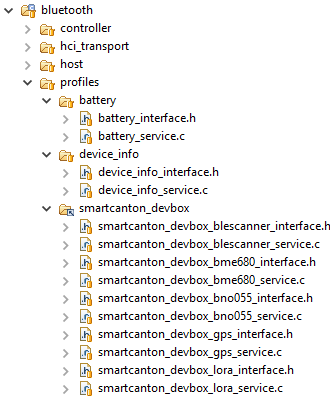
\includegraphics[width=0.50\textwidth]{Figures/Software/kw41z/ble_services_paths.png}
    \caption{Fichiers de déclaration des services Bluetooth}
    \label{fig-ble_services_paths}
\end{figure}



% ---------------------------------------------------------------------------------------------%
\FloatBarrier
\subsubsubsection{Fonctions minimales d'un profil}
% ---------------------------------------------------------------------------------------------%

Sur le KW41Z, deux méthodes doivent être implémentées dans chaque profil. La première est la fonction start qui sera appelée lors de l'initialisation de l'application, avec la réception de l'événement \path{gInitializationComplete_c} dans le \textit{callback} de l'hôte, nommé \path{BleApp_GenericCallback} : 

\begin{tcolorbox}
  [top=-1mm, bottom=-3mm, left=0mm, right=0mm, enhanced,breakable,
  attach boxed title to top center={yshift=-3mm,yshifttext=-1mm},colback=LightGray,colframe=DarkGray,
  colbacktitle=DarkGray, fonttitle=\footnotesize\bfseries,boxed title style={size=small,colframe=DarkGray},
  title=\texttt{dev\_box\_app\_task.c}]


\cfile[firstline=536,lastline=537]{SourceCode/dev_box_app_task.c}
...
\cfile[firstline=559,lastline=559]{SourceCode/dev_box_app_task.c}
\end{tcolorbox}

L'unique but de cette fonction est d'initialiser l'ID du périphérique connecté avec la valeur \texttt{gInvalidDeviceId\_c}. Les deux autres fonctions se nomment \texttt{subscribe} et \texttt{unsubscribe}.
L'objectif de celles-ci est d'enregistrer la connexion au service d'un nouveau maitre et informer les applications, qui doivent diffuser des données, que quelqu'un est peut-être intéressé à les recevoir. L'ID est simplement stockée en local dans le profil et est libéré lorsque le maitre se déconnecte : 
\begin{tcolorbox}
  [top=-1mm, bottom=-3mm, left=0mm, right=0mm, enhanced,breakable,
  attach boxed title to top center={yshift=-3mm,yshifttext=-1mm},colback=LightGray,colframe=DarkGray,
  colbacktitle=DarkGray, fonttitle=\footnotesize\bfseries,boxed title style={size=small,colframe=DarkGray},
  title=\texttt{smartcanton\_devbox\_gps\_service.c} ]
  

\cfile[firstline=79,lastline=85]{SourceCode/smartcanton_devbox_gps_service.c}
...
\cfile[firstline=87,lastline=92]{SourceCode/smartcanton_devbox_gps_service.c}
\end{tcolorbox}

Aucun exemple prodigué par NXP ne supporte le multi maitre. Cependant, la \textit{datasheet} du KW41Z spécifie que deux maitres peuvent être connectés simultanément. On peut voir que cette implémentation n'est pas pensée pour gérer deux connexions. Toutefois, pour la DevBox, cette multiple connexion n'a pas été activée dans les options du SDK, car elle n'a pas forcément de sens pour le projet.


% ---------------------------------------------------------------------------------------------%
\FloatBarrier
\subsubsubsection{Écritures et lecture depuis la base de donnée GATT}
% ---------------------------------------------------------------------------------------------%

La base de donnée GATT est régie par une suite d'interfaces très complètes contenues dans le répertoire \path{<project_name>/bluetooth/interface/}. Lorsque l'utilisateur souhaite sauvegarder des données dans la table GATT, il dispose d'une fonction nommée \textit{GattDb\_WriteAttribute}. L'entête de cette fonction est disponible ci-dessous:

\begin{tcolorbox}
  [top=-1mm, bottom=-3mm, left=0mm, right=0mm, enhanced,breakable,
  attach boxed title to top center={yshift=-3mm,yshifttext=-1mm},colback=LightGray,colframe=DarkGray,
  colbacktitle=DarkGray, fonttitle=\footnotesize\bfseries,boxed title style={size=small,colframe=DarkGray},
  title=\texttt{gatt\_db\_app\_interface.h} ]
\inputminted[firstline=78,lastline=83,bgcolor=LightGray,fontsize=\footnotesize,breaklines,linenos]{C}{SourceCode/gatt_db_app_interface.h}
\end{tcolorbox}

Le premier paramètre est l'\textit{handle} de la caractéristique du service désiré à l'aide d'une fonction nommée \path{GattDb_FindCharValueHandleInService}. La nouvelle valeur de la caractéristique est ensuite écrite à l'aide des deux paramètres suivants. Si les données écrites sont fausses ou que la caractéristique est invalide, la fonction retourne une erreur. La lecture est également réalisée à l'aide d'une fonction du même fichier, en spécifiant des paramètres similaires : 
\begin{tcolorbox}
  [top=-1mm, bottom=-3mm, left=0mm, right=0mm, enhanced,breakable,
  attach boxed title to top center={yshift=-3mm,yshifttext=-1mm},colback=LightGray,colframe=DarkGray,
  colbacktitle=DarkGray, fonttitle=\footnotesize\bfseries,boxed title style={size=small,colframe=DarkGray},
  title=\texttt{gatt\_db\_app\_interface.h} ]
\inputminted[firstline=99,lastline=105,bgcolor=LightGray,fontsize=\footnotesize,breaklines,linenos]{C}{SourceCode/gatt_db_app_interface.h}
\end{tcolorbox}

% ---------------------------------------------------------------------------------------------%
\FloatBarrier
\subsubsubsection{Notifications}
% ---------------------------------------------------------------------------------------------%

Dans le cadre de ce projet, uniquement les notifications ont été implémentées. Les indications sont plus complexes à mettre en place, car il faut créer manuellement des machines d'états et des \textit{queues} pour l'envoi et ensuite l'attente de la confirmation (cf. \cref{sec-protocols_BLE_services} pour la différence entre notifications et indications). Les notifications n'ont jamais été utilisées avec des données critiques où l'ont doit être sûr d'avoir la réception sur le maitre, cet \textit{overhead} était alors inutile dans ce projet.\\

Une fois les données des caractéristiques enregistrées dans la base de données avec la fonction \path{GattDb_WriteAttribute}, celles-ci peuvent être notifiées aux clients qui se sont enregistrés en écrivant dans le CCCD. Cette opération de notification est activée à l'aide de la fonction \path{GattServer_SendNotification} : 

\begin{tcolorbox}
  [top=-1mm, bottom=-3mm, left=0mm, right=0mm, enhanced,breakable,
  attach boxed title to top center={yshift=-3mm,yshifttext=-1mm},colback=LightGray,colframe=DarkGray,
  colbacktitle=DarkGray, fonttitle=\footnotesize\bfseries,boxed title style={size=small,colframe=DarkGray},
  title=\texttt{gatt\_server\_interface.h} ]
\inputminted[firstline=268,lastline=272,bgcolor=LightGray,fontsize=\footnotesize,breaklines,linenos]{C}{SourceCode/gatt_server_interface.h}
\end{tcolorbox}

Le premier paramètre spécifié est l'identifiant du maitre et le deuxième est l'\textit{handle} de la caractéristique. 

Lorsque le flux des données est trop important, il est inutile de les sauvegarder. Cela affecte les performances du microcontrôleur puisque celles-ci doivent être à chaque fois copiées dans la base de données. Par exemple, dans le cas de la capture des données provenant d'un accéléromètre, la fréquence d'acquisition peut attendre plusieurs centaines d'Hertz ce qui crée des écritures inutiles dans la base de données. Le framework propose donc la possibilité de notifier l'utilisateur sans sauvegarder les informations. Ceci s'effectue à l'aide de la fonction \path{GattServer_SendInstantValueNotification}. Voici l'entête de cette fonction : 

\begin{tcolorbox}
  [top=-1mm, bottom=-3mm, left=0mm, right=0mm, enhanced,breakable,
  attach boxed title to top center={yshift=-3mm,yshifttext=-1mm},colback=LightGray,colframe=DarkGray,
  colbacktitle=DarkGray, fonttitle=\footnotesize\bfseries,boxed title style={size=small,colframe=DarkGray},
  title=\texttt{gatt\_server\_interface.h} ]
\inputminted[firstline=302,lastline=308,bgcolor=LightGray,fontsize=\footnotesize,breaklines,linenos]{C}{SourceCode/gatt_server_interface.h}
\end{tcolorbox}

Les paramètres sont similaires à la fonction précédente, mais cette fois, la nouvelle doit être spécifiée lors de l'appel. Cette fonction a été utilisée dans ce projet pour tous les services Bluetooth qui ont des caractéristiques listées comme étant uniquement accessibles en tant que notifications (ex. les données du BNO055, cf. \cref{sec-software_ble_services_bno055}). Le KW41Z ne supporte qu'au maximum 16 notifications par maitre connecté et ce chiffre affecte directement toutes les notifications, même si le maitre ne s'abonne pas à celles-ci. Cette limitation ne peut pas être modifiée, cela a donc limité le nombre de caractéristiques qui ont pu être assignées comme notifications pour l'ensemble du projet.

% ---------------------------------------------------------------------------------------------%
\FloatBarrier
\subsubsection{Services BLE disponibles sur la DevBox}
\label{sec-software_ble_services}
% ---------------------------------------------------------------------------------------------%

La documentation de tous les services Bluetooth implémentés dans ce projet est disponible en \cref{AppendixBluetoothServices} sous forme de tableaux décrivant tous les UUIDs, les droits d'accès ainsi que des exemples de données fournies par les divers services. Les quatre sous-sections qui suivent expliquent plus en détail les différents services, de même que leurs rôles dans ce projet. Ces services peuvent ainsi être accédés par n'importe quel client BLE, par exemple, en utilisant l'application NRF Connect sur Android (cf. \cref{fig-nrf_connect_gps}).


\begin{figure}[ht!]
    \centering
    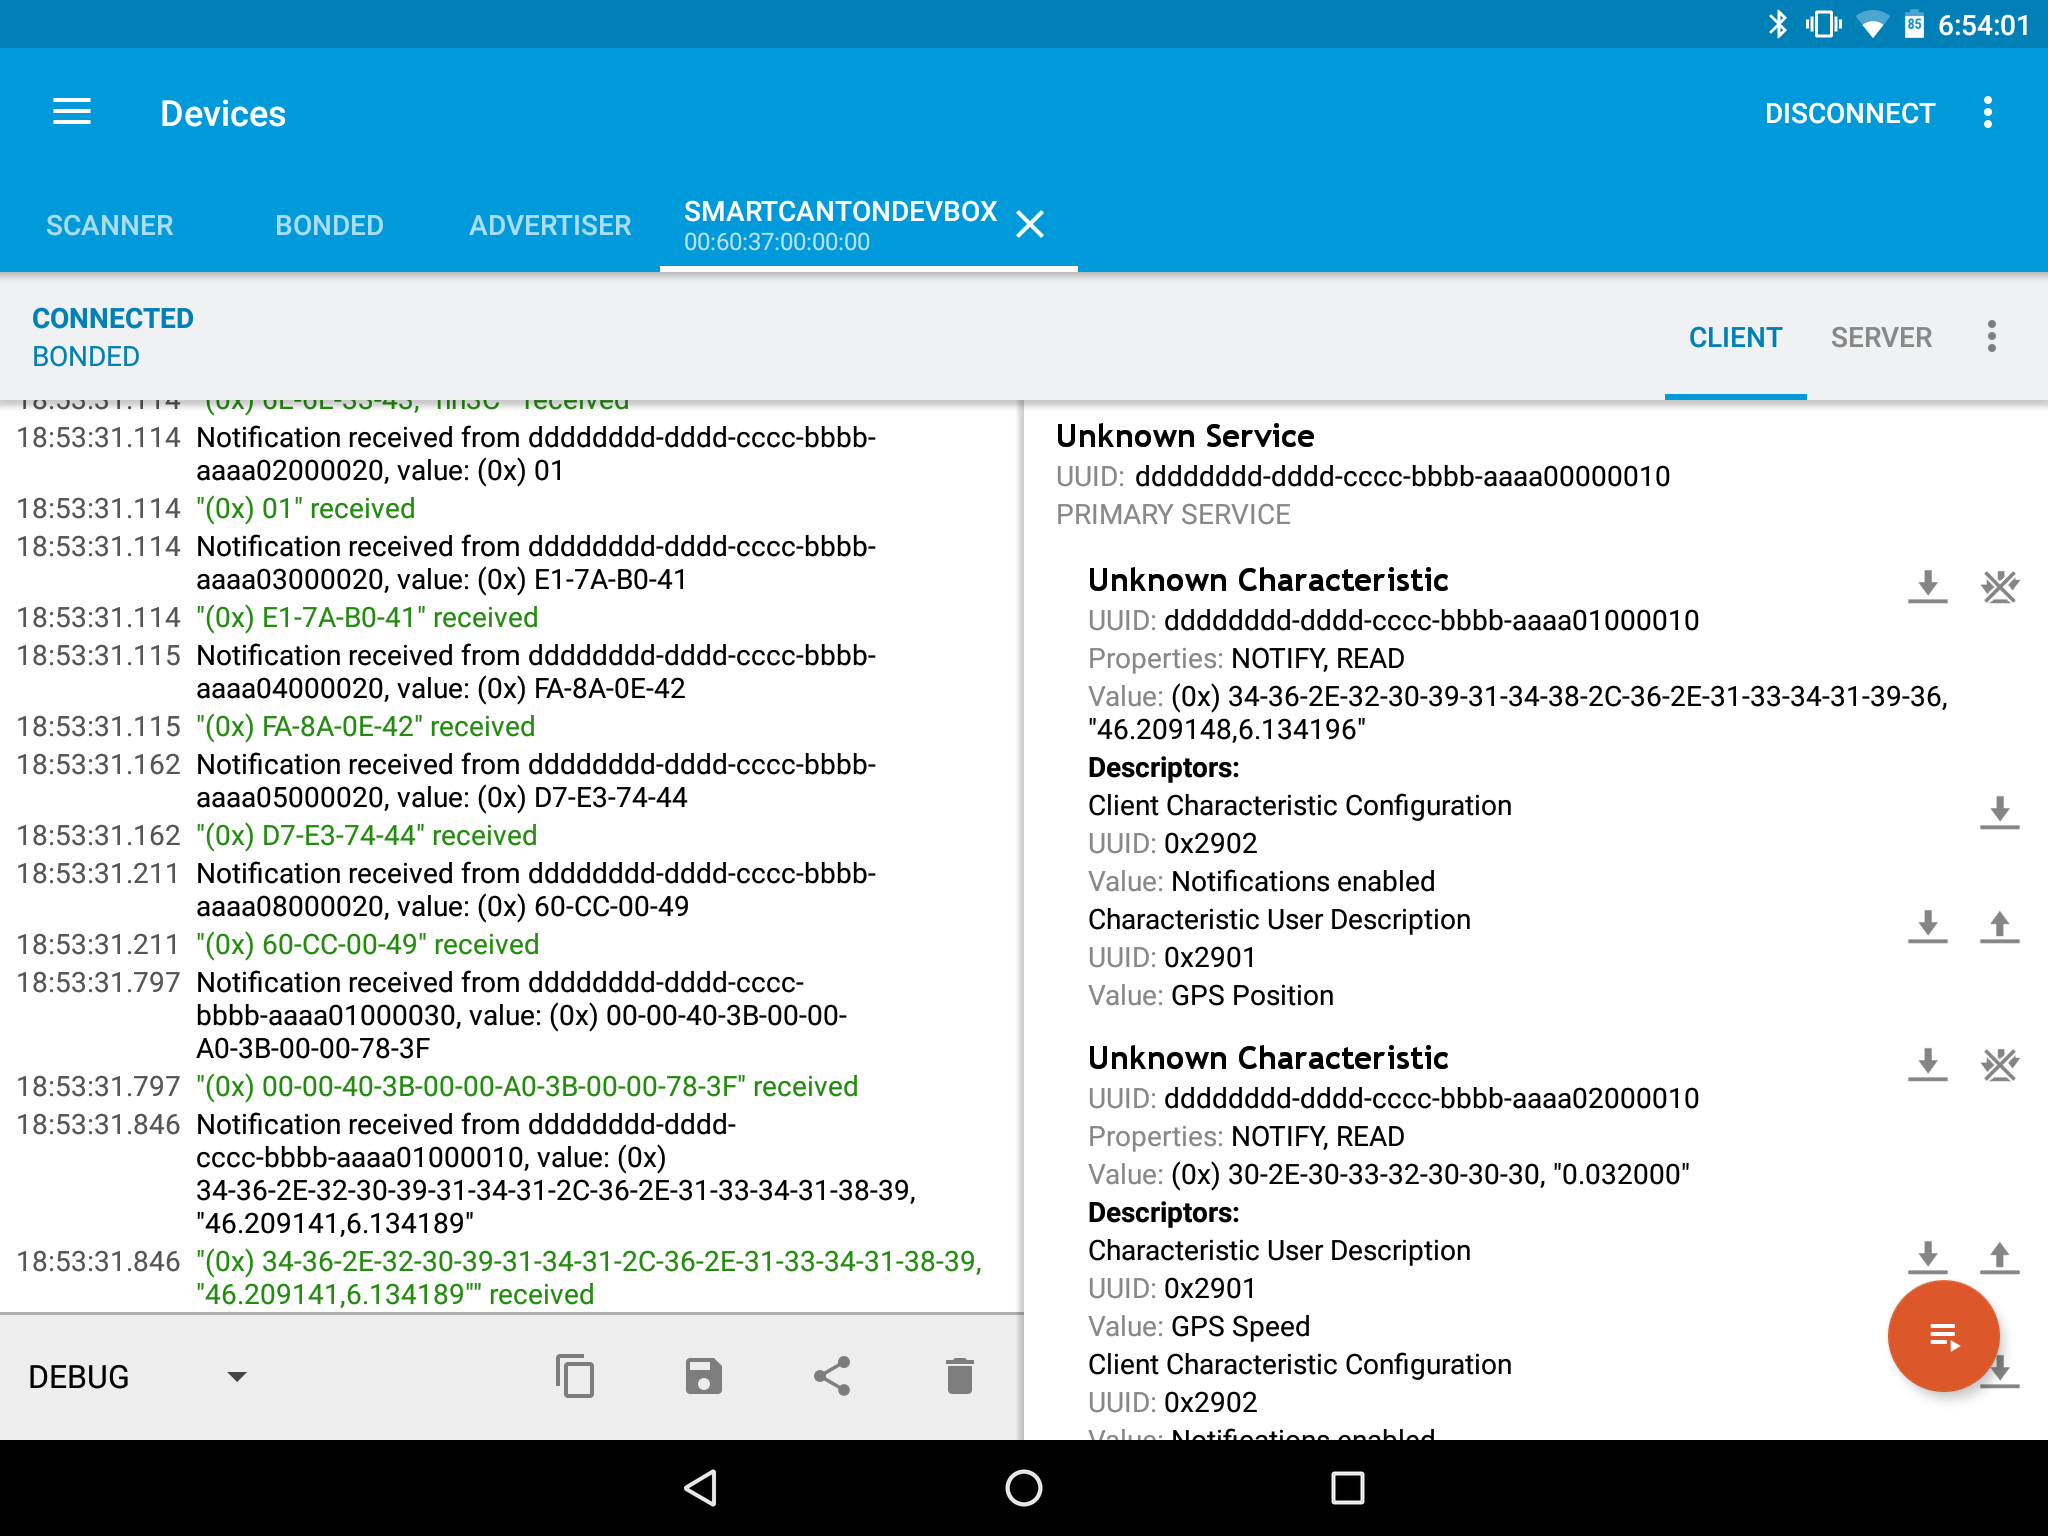
\includegraphics[width=0.9\textwidth]{Figures/Software/kw41z/nrf_connect_gps.png}
    \caption{Lecture des caractéristiques du service de GPS à l'aide de l'application \textit{NRF Connect}}
    \label{fig-nrf_connect_gps}
\end{figure}


% ---------------------------------------------------------------------------------------------%
\FloatBarrier
\subsubsubsection{\textit{Generic Access}, \textit{Generic Attribute} et \textit{Battery}}
% ---------------------------------------------------------------------------------------------%

Ces trois services utilisent les profils Bluetooth standards et n'ont donc pas été modifiés pour être utilisés sur ce projet. \texttt{Generic Access} permet uniquement d'indiquer quelques informations sur le périphérique connecté, comme les différentes versions du \textit{firmware}, \textit{hardware} ou le constructeur. Il peut ainsi être utilisé par le maitre pour garantir que le périphérique connecté est bien une DevBox et non un autre périphérique. Le contenu de ces services est visible en annexe sur le \cref{tab-GenericAccessService}, \cref{tab-GenericAttributeService} et \cref{tab-BatteryService}.\\

Le service de batterie est celui qui est fourni par l'exemple \textit{Hearth Rate Sensor} de NXP. Pour notifier l'état de la batterie, c'est l'application qui actualise la valeur de celle-ci toutes les 30 secondes à l'aide d'un \textit{timer}. Cette mise à jour s'effectue dans la tâche principale du projet (DevBox Main Task).


% ---------------------------------------------------------------------------------------------%
\FloatBarrier
\subsubsubsection{SmartCanton DevBox LoRaWAN}
% ---------------------------------------------------------------------------------------------%

Ce service est l'un des plus importants de la DevBox, car il permet la mise à jour des différents paramètres de la connexion LoRaWAN. Les opérations autorisées sur les différentes caractéristiques sont décrites sur le \cref{tab-SmartCantonLoRaService} en annexe. Sur ce tableau, les caractéristiques listées avec le tag \texttt{[DEBUG]} signifient que celles-ci ne sont accessibles que pour le développement actuel. Elles sont placées en lecture seule si la DevBox doit être utilisée pour un cas d'utilisation définitif. Voici une liste des différentes caractéristiques implémentées : 
\begin{enumerate}
    \item LoRaWAN App EUI;
    \item LoRaWAN AppKey; 
    \item LoRaWAN Device EUI;
    \item LoRaWAN mode de confirmation des paquets (confirmés ou non);
    \item LoRaWAN statu du réseau (rejoint ou non);
    \item LoRaWAN \textit{Device Address} assignée par le réseau;
    \item LoRaWAN Network Session Key;
    \item LoRaWAN App Session Key;
    \item Validation de la configuration appliquée. Cette dernière option permet de valider une configuration une fois que toutes les caractéristiques ont été écrites. Celle-ci va annuler la configuration actuelle du module LoRaWAN afin d'appliquer la dernière configuration entrée par l'utilisateur.  
\end{enumerate}


% ---------------------------------------------------------------------------------------------%
\FloatBarrier
\subsubsubsection{SmartCanton DevBox GPS}
% ---------------------------------------------------------------------------------------------%

Le service Bluetooth implémenté pour le GPS permet de recevoir les différentes informations provenant de celui-ci. A l'heure actuelle, uniquement les données des trames de type RMC sont supportées \cite{NMEAdata3:online}. 

Toutes les informations sont disponibles en tant que notifications. Comme le débit n'est pas très élevé (une fois par seconde), la dernière valeur de chaque caractéristique est stockée dans la base de données. Ceci permet également de savoir quand la dernière valeur GPS a pu être capturée (que ce soit la position ou le temps). Voici la liste des différentes caractéristiques qui ont été implémentées : 
\begin{enumerate}
    \item Position avec la latitude et longitude en degrés;
    \item Vitesse en m/s;
    \item Trajectoire;
    \item Date en format \texttt{hh:mm:ss};
    \item Heure en format \texttt{hh:mm:ss}.
\end{enumerate}

Le service complet est disponible sur le \cref{tab-SmartCantonGPSService} en annexe. Pour simplifier le débogage, les données sont toutes en format string UTF8. Le traitement rajouté sur les données est faible, car elles sont en partie récupérées sous ce format directement depuis la trame RMC transmise par le GPS. Cela alourdit l'envoi à travers la communication Bluetooth, mais le débit qui est actuellement d'une trame par seconde reste négligeable.


% ---------------------------------------------------------------------------------------------%
\FloatBarrier
\subsubsubsection{SmartCanton DevBox BME680}
% ---------------------------------------------------------------------------------------------%

Le capteur de température, d'humidité, de pression et de qualité de l'air dispose d'un grand nombre de données accessibles. Cependant, puisque le KW41Z ne supporte que 16 caractéristiques en notifications, des concessions ont été faites sur les flux de données disponibles. Voici la liste des caractéristiques implémentées : 
\begin{enumerate}
    \item \textit{Indoor Air Quality} (IAQ) facteur de 0 à 400;
    \item Qualité de l'IAQ en échelle de 0 à 3 (0 : données inutilisables et une calibration est nécessaire, 3 : capteur parfaitement calibré et données parfaites);
    \item Température en °C;
    \item Humidité en \,\%;
    \item Pression en hPa;
    \item Température brute en °C (sans le post traitement de la bibliothèque BSEC);
    \item Humidité brute en \,\% (sans le post traitement de la bibliothèque BSEC);
    \item Mesure du GAS brut en ohms (sans le post traitement de la bibliothèque BSEC).
\end{enumerate}

Le service complet est disponible sur le \cref{tab-SmartCantonBME680Service} en annexe.

% ---------------------------------------------------------------------------------------------%
\FloatBarrier
\subsubsubsection{SmartCanton DevBox BNO055}
\label{sec-software_ble_services_bno055}
% ---------------------------------------------------------------------------------------------%

Le BNO055 peut fournir beaucoup de données, mais il a été décidé de seulement garder l'accès aux trois capteurs principaux (accéléromètre, gyroscope et magnétomètre). Voici la liste des caractéristiques implémentées : 
\begin{enumerate}
    \item Trois axes de l'accéléromètre en g codé chacun sur 4 bytes pour un total de 12 bytes;
    \item Trois axes du gyroscope en degrés par secondes codé chacun sur 4 bytes pour un total de 12 bytes;
    \item Trois axes du magnétomètre en microtesla codé chacun sur 4 bytes pour un total de 12 bytes;
    \item Le temps entre chaque nouvelle mesure. L'utilisateur peut choisir un temps de 300 à 10000 ms pour être à nouveau notifié.
\end{enumerate}

Le service complet est disponible sur le \cref{tab-SmartCantonBNO055Service} en annexe. Actuellement l'envoi des données n'est pas optimisé pour les grands débits, c'est pour cela que la configuration entre chaque mesure est limitée à 300ms. Pour pallier à cette limitation, il faut envoyer plusieurs échantillons dans une même notification afin d'éviter l'\textit{overhead} généré par les paquets BLE.

% ---------------------------------------------------------------------------------------------%
\FloatBarrier
\subsubsubsection{SmartCanton DevBox BLE Scanner}
% ---------------------------------------------------------------------------------------------%

Le scanneur Bluetooth est basique, il ne propose actuellement pas beaucoup de personnalisation. Voici la liste des caractéristiques implémentées : 
\begin{enumerate}
    \item Nombre de périphériques scannés lors de la dernière fenêtre de capture;
    \item Le temps entre chaque nouvelle fenêtre de capture. L'utilisateur peut choisir un temps de 10 à 600 secondes pour être à nouveau notifié.
\end{enumerate}

Le service complet est disponible sur le \cref{tab-SmartCantonBLEScannerService} en annexe.


\subsection{Sécurité}
\label{sec-smartcanton_devbox_security}

La \textit{stack} BLE du KW41Z s'occupe d'une grande partie de la sécurité en interne. Les sous-sections qui suivent expliquent les différents paramètres configurés afin de suivre les recommandations du NIST citées en \cref{sec-security_ble_recommendatiions}.\\


La méthode d'authentification retenue a été le \textit{passkey}. Celui-ci est généré aléatoirement pour chaque DevBox et programmé dans celle-ci. En section \cref{sec-security_ble}, il a été vu que si un périphérique souhaite forcer l'utilisation d'un \textit{passkey}, il doit indiquer qu'il dispose d'un écran pour afficher ce dernier, même si cette information est fausse. Cela aura pour conséquence de forcer l'initiateur de la connexion à demander un \textit{passkey}. Cette demande de \textit{passkey} ne s'effectue que si l'initiateur dispose d'un écran et d'un clavier, ce qui est le cas pour un smartphone. Si ce n'est pas le cas, la connexion est refusée, car le mode 1 niveau 4 a été activé et exigeant une connexion authentifiée et sécurisée. 
Le NIST (cf. \cref{sec-security_ble_recommendatiions}) conseille uniquement de ne pas utiliser de \textit{passkey} simple. Dans le cas présent, le \textit{passkey} est différent pour chaque périphérique. Le \textit{passkey} est ensuite uniquement accessible sur un serveur sécurisé. On peut voir cela comme un autre type d'échange d'information de type Out Of the Band (OOB). La solution la plus sure serait d'échanger directement vraies LTK Bluetooth à l'aide du serveur et de les programmer dans le dispositif souhaitant se connecter sur la DevBox. Toutefois, dans ce projet un smartphone a été utilisé, et ce type d'injection de clés n'est pas possible dans Android sans être en mode développeur ou root \cite{Gettingt47:online}.\\

Si l'attaquant arrive à \textit{brute force} le \textit{passkey}, celui-ci peut alors se connecter sur le périphérique. Toutefois, celui-ci ne peut pas lire les clés, car celles-ci sont en lecture seules. Il peut tout de même modifier certains paramètres et également changer le périphérique de réseau LoRaWAN. Néanmoins, dans un cas comme celui-là, une alerte via un message \textit{uplink} LoRa peut être générée pour indiquer une nouvelle connexion Bluetooth.


\subsubsection{Adresses MAC Bluetooth}

Les adresses MAC doivent être uniques pour tous les périphériques Bluetooth. Celle-ci doit être configurée manuellement à l'aide de la macro \path{BD_ADDR} : 

\begin{tcolorbox}
  [top=-1mm, bottom=-3mm, left=0mm, right=0mm, enhanced,breakable,
  attach boxed title to top center={yshift=-3mm,yshifttext=-1mm},colback=LightGray,colframe=DarkGray,
  colbacktitle=DarkGray, fonttitle=\footnotesize\bfseries,boxed title style={size=small,colframe=DarkGray},
  title=\path{app_preinclude.h} ]
\inputminted[firstline=155,lastline=155,bgcolor=LightGray,fontsize=\scriptsize,breaklines,linenos]{C}{SourceCode/app_preinclude.h}
\end{tcolorbox}

NXP ne fournit pas d'adresses MAC pour les périphériques. Celles-ci doivent être achetées auprès des autorités d'assignation régies par l'IEEE\footnote{\url{https://standards.ieee.org/develop/regauth/grpmac/index.html}}. Les recommandations du NIST (cf. \cref{sec-security_ble_recommendatiions}) demandent de garder une trace de toutes ces adresses MAC. Donc par cet achat, cela permet de connaitre la plage d'adresses MAC assignée aux différents périphériques vendus ou développés.

\subsubsection{Sécurité des services Bluetooth}

La sécurité des services Bluetooth a été placée en suivant les recommandations du NIST exposées en \cref{sec-security_ble_recommendatiions}. Il s'agit de mettre la sécurité en Mode 1 et Level 3. La stack Bluetooth du KW41Z est configurée avec les des différents paramètres qui suivent : 

\newpage
\begin{tcolorbox}
  [top=-1mm, bottom=-3mm, left=0mm, right=0mm, enhanced,breakable,
  attach boxed title to top center={yshift=-3mm,yshifttext=-1mm},colback=LightGray,colframe=DarkGray,
  colbacktitle=DarkGray, fonttitle=\footnotesize\bfseries,boxed title style={size=small,colframe=DarkGray},
  title=\path{app_config.c} ]
\inputminted[firstline=166,lastline=181,bgcolor=LightGray,fontsize=\scriptsize,breaklines,linenos]{C}{SourceCode/app_config.c}
\end{tcolorbox}

La \textit{stack} Bluetooth permet également de mettre en place des niveaux de sécurité personnalisés pour trois services à l'aide de l'option \path{aServiceSecurityRequirements}. Si aucun service n'est spécifié dans cette personnalisation, c'est la configuration \path{pMasterSecurityRequirements} qui est appliquée à tous les services. Cette option de sécurité personnalisée n'a pas été utilisé dans ce projet, mais on peut imaginer laisser un service sans sécurité, afin d'informer les utilisateurs d'informations non critiques concernant le périphérique.

\subsubsection{\textit{Passkey} Bluetooth Low Energy}

Le \textit{passkey} du Bluetooth doit être généré lors de la programmation des cartes DevBox. La définition de celui-ci s'effectue à l'aide de la ligne suivante : 
\begin{tcolorbox}
  [top=-1mm, bottom=-3mm, left=0mm, right=0mm, enhanced,breakable,
  attach boxed title to top center={yshift=-3mm,yshifttext=-1mm},colback=LightGray,colframe=DarkGray,
  colbacktitle=DarkGray, fonttitle=\footnotesize\bfseries,boxed title style={size=small,colframe=DarkGray},
  title=\path{app_preinclude.h} ]
\inputminted[firstline=35,lastline=36,bgcolor=LightGray,fontsize=\scriptsize,breaklines,linenos]{C}{SourceCode/app_preinclude.h}
\end{tcolorbox}

Le \textit{passkey} doit être de minimum 6 digits et doit être unique pour chaque DevBox. Il n'y a actuellement pas d'autre possibilité de le changer à l'exception de cette ligne de code. Malheureusement, il n'est pas possible de suivre la recommandation du NIST au sujet du \textit{passkey} aléatoire à chaque connexion (cf. \cref{sec-security_ble_recommendatiions}).

\subsubsection{Stockage des clés LoRaWAN}

Dans l'idéal, les clés LoRaWAN doivent être stockées dans le module LoRaWAN. Cependant, l'implémentation n'a pas pu être faite dans le temps imparti à ce travail. À l'heure actuelle, les clés sont stockées dans le microcontrôleur KW41Z en flash à l'aide de la structure \path{lorawanControllerConfiguration_t} présentée en \cref{sec-softawre_kw41z_libs_lorawan_controller}.



\FloatBarrier
\newpage
\section{Application Android SmartCanton Manager}
\label{sec-soft_android}


L'application Android, nommée SmartCanton Manager, a pour but de créer un pont entre deux technologies, comme illustré en \cref{fig-diagram_android_architecture} mais également de créer un canal d'échange sécurité pour le transfert de l'AppKey LoRaWAN. 

L'application offre également la possibilité de tester les différents capteurs présents sur une DevBox en se connectant aux différents services Bluetooth présentés en \cref{sec-software_ble_services}. La récupération des données s'effectue à l'aide de lectures BLE ou via des flux de notifications BLE.

\begin{figure}[ht!]
    \centering
    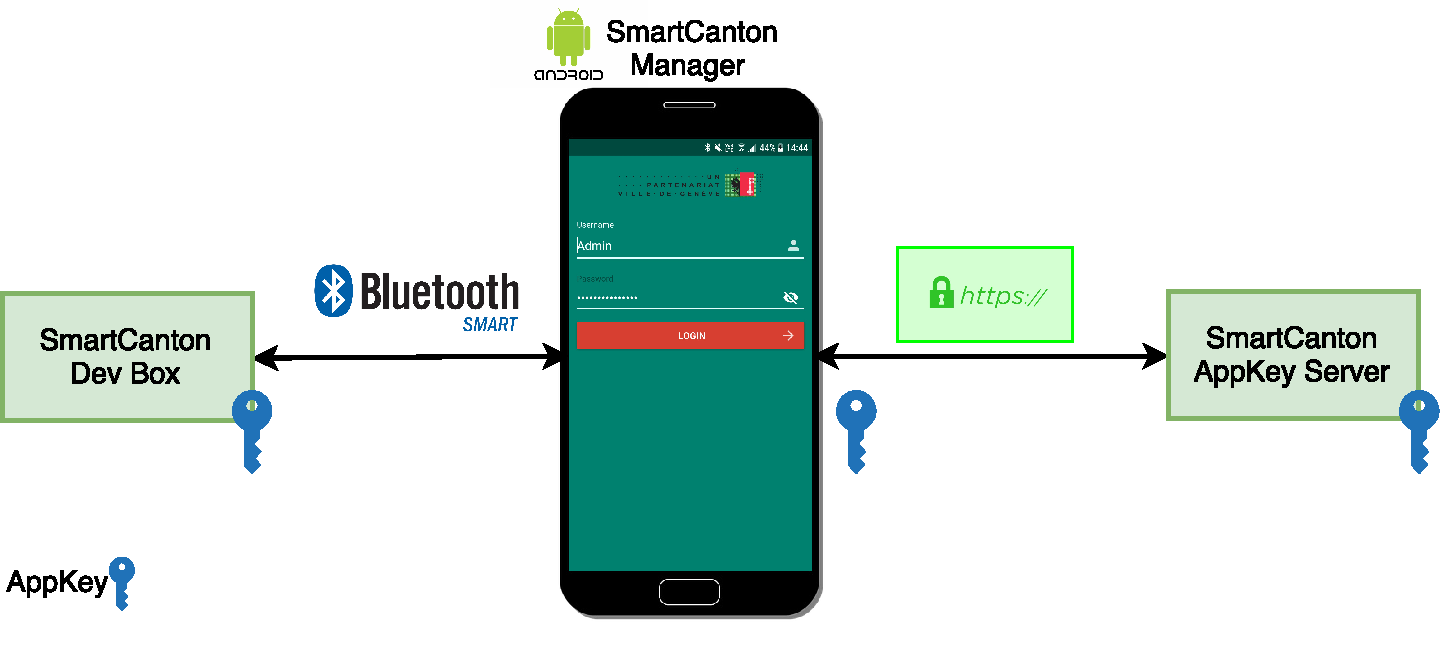
\includegraphics[width=1.0\textwidth]{Figures/Software/diagram_android_architecture.pdf}
    \caption{Rôle de l'application mobile}
    \label{fig-diagram_android_architecture}
\end{figure}


\subsection{Frameworks utilisés}

Afin d'accélérer la programmation sur Android, deux frameworks majeurs ont été utilisés. Ceux-ci sont listés dans les sous-sections qui suivent.

\subsubsection{SweetBlue}

Android est censé s'abstraire du matériel afin d'offrir une interface générique pour chaque plateforme utilisée, surtout sur les smartphones. Néanmoins, le comportement du Bluetooth diffère encore entre les différents périphériques Android utilisés. Par exemple, Samsung bride la fréquence des scans Bluetooth possible sur ses smartphones lorsque ceux-ci sont verrouillés. Cette décision a été prise pour réduire la consommation énergétique des applications qui s'exécutent en arrière-plan sur un smartphone. Ceci n'est pas le cas sur la plupart des autres constructeurs. La \textit{stack} Bluetooth sur Android est également très \textit{bas niveau}. Par exemple, si on souhaite lire plusieurs caractéristiques BLE à la suite, l'utilisateur doit lui-même créer une file de lecture avec la gestion de toutes les erreurs, car deux lectures ne peuvent pas être effectuées en parallèle. Voici une liste complète des divers problèmes qui sont aujourd'hui encore non résolus sur les diverses versions d'Android :
\begin{center}
    \url{https://github.com/iDevicesInc/SweetBlue/wiki/Android-BLE-Issues}
\end{center}

Pour pallier à cela, une bibliothèque nommée SweetBlue a été développée par l'entreprise iDevicesInc\footnote{\url{https://idevicesinc.com/sweetblue/}}. Celle-ci a pour but de simplifier l'intégration du Bluetooth dans une application et d'essayer de corriger certaines instabilités. La bibliothèque est gratuite dans son intégralité pour un usage privé même si l'application finale n'est pas vendue à des utilisateurs.


\subsubsection{Retrofit}

Sur Android, la gestion des appels asynchrones peut vite devenir compliquée et répétitive. Retrofit est un client \textit{type-safe} pour les API REST sur Java, avec un accent prononcé pour Android. Cette bibliothèque est développée par l'entreprise Square\footnote{\url{http://square.github.io/retrofit/}}, spécialisée dans les logiciels \textit{open sources}. Cette bibliothèque fournit un framework complet et simple à utiliser pour interagir avec les APIs et recevoir des requêtes avec le client OkHttp\footnote{\url{http://square.github.io/okhttp/}}.

La gestion des erreurs HTTP sont directement traitées par le framework à l'aide de \textit{callbacks} avec les méthodes \texttt{success} et \texttt{failure}.


\subsection{Manuel d'utilisation de l'application}

L'\cref{AppendixAndroidAppUserGuide} contient un manuel d'utilisation de l'application Android. Avec toutes les étapes qui sont nécessaires pour se connecter au serveur, lister les périphériques Bluetooth à proximité, ainsi que la connexion avec ces derniers.


\subsection{Activités}

 Pour ne pas surcharger la présentation de cette section, toutes les captures d'écran de l'application sont présentées dans le manuel d'utilisateur situé à l'\cref{AppendixAndroidAppUserGuide}.
 
 
\begin{figure}[ht!]
    \centering
    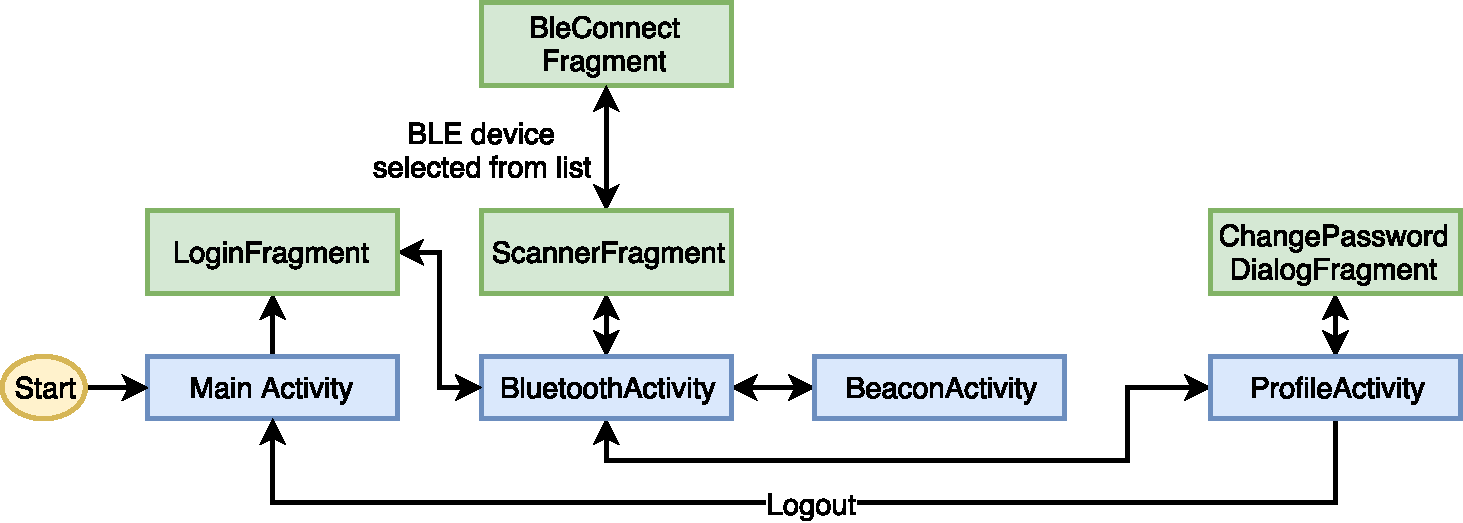
\includegraphics[width=1.0\textwidth]{Figures/Software/diagram_android_activites.pdf}
    \caption{Diagramme d'interconnexions entre les différentes activités Android}
    \label{fig-diagram_android_activites}
\end{figure}


L'architecture générale de l'application avec la présentation des diverses activités et fragments est visible sur la \cref{fig-diagram_android_activites}. On constate que l'application n'est composée que de quatre activités. Voici leurs différents rôles :
\begin{itemize}
    \item \texttt{MainActivity} : affiche le fragment \texttt{LoginFragment} qui offre la possibilité à l'utilisateur de s'authentifier auprès du serveur, afin de recevoir un \textit{token} JWT (cf. \cref{fig_apdx-login_activity}). Une fois le login accepté, l'activité \texttt{BluetoothActivity} est appelée.
    \item \texttt{BluetoothActivity} : gère les diverses communications Bluetooth entre les différents périphériques. Cette activité peut afficher deux fragments :
        \begin{enumerate}
            \item \texttt{ScannerFragment} : fragment instancié par défaut au démarrage de l'activité et a pour but de lister tous les périphériques Bluetooth Low Enerny à proximité (cf. \cref{fig_apdx-bluetooth_scanner_frag}). Les dispositifs sont affichés dans une liste et peuvent être sélectionnés par l'utilisateur.
            \item \texttt{BleConnectFragment} : fragment affiché lorsque l'utilisateur sélectionne un périphérique. Lors du chargement du fragment, une requête vers le serveur est automatiquement envoyée afin de savoir si le dispositif est connu en fonction de l'adresse MAC de ce dernier. Si le périphérique est connu, l'utilisateur peut se connecter au périphérique via Bluetooth et ainsi accéder aux divers périphériques (cf. \cref{fig_apdx-ble_dev_connection_process}). Il peut également mettre à jour le périphérique avec les dernières configurations LoRaWAN contenues sur le serveur.
        \end{enumerate}
    \item \texttt{BeaconActivity} : ne contient pas de fragment, car elle n'a qu'un seul et unique rôle, qui est de générer un certain nombre de \textit{beacons} afin de simuler des périphériques Bluetooth Low Energy à proximité comme vu en \cref{sec-software_scanner_ble}.
    \item \texttt{ProfileActivity} : Cette activité permet d'afficher les informations sur l'utilisateur connecté, ainsi que sur le \textit{token} JWT récupéré lors de la connexion. Ici l'utilisateur peut également se déconnecter de sa session (cf. \cref{fig_apdx-profile_activity}).
\end{itemize}



\subsection{Sécurité}


Pour ce qu'il s'agit de la sécurité, tout est directement géré par Android même. Dans le cas des requêtes HTTPS, il suffit de spécifier que l'URL du serveur est en HTTPS pour que toute la communication soit automatiquement chiffrée à l'aide du certificat fournit par le serveur. \\

Dans le cas du Bluetooth, c'est le périphérique qui décide du mode de sécurité qu'il accepte (cf. \cref{sec-security_ble}). Android s'occupe donc d'effectuer la connexion avec requêtes de celui-ci. La demande de \textit{passkey} est demandée directement par l'OS et ne peut pas être directement validée par l'application. Pour informer l'utilisateur sur la présence du \textit{passkey}, une popup est affichée lors de la connexion dévoilant ainsi le PIN que l'utilisateur doit rentrer sur le périphérique (cf. \cref{fig_apdx-ble_dev_connected_startup}).


\FloatBarrier
\newpage
\section{Serveur de management de SmartCanton DevBox}
\label{sec-soft_server}

Pour stocker les diverses informations sur les périphériques DevBox, et gérer les utilisateurs, un serveur avec une API REST\footnote{\url{https://en.wikipedia.org/wiki/Representational_state_transfer}}, ainsi qu'une base de données SQLite\footnote{\url{https://en.wikipedia.org/wiki/SQLite}} ont été mis en place. Un digramme illustrant la connexion est visible à l'aide de la \cref{fig-diagram_architecture_rest_api}).
En utilisant une API REST, le développeur final peut utiliser la platefrome avec laquelle il est le plus à l'aise. Dans le cadre de ce travail, c'est une application Android qui a été utilisée lors de la communication. Contrairement à la mise à disposition d'une base de données directe, l'API laisse une plus grande flexibilité lorsque des modifications sur les tables doivent être faites au fur et à mesure de l'avancement d'un projet, et ceci sans affecter le code précédemment implémenté par les développeurs.

\begin{figure}[ht!]
    \centering
    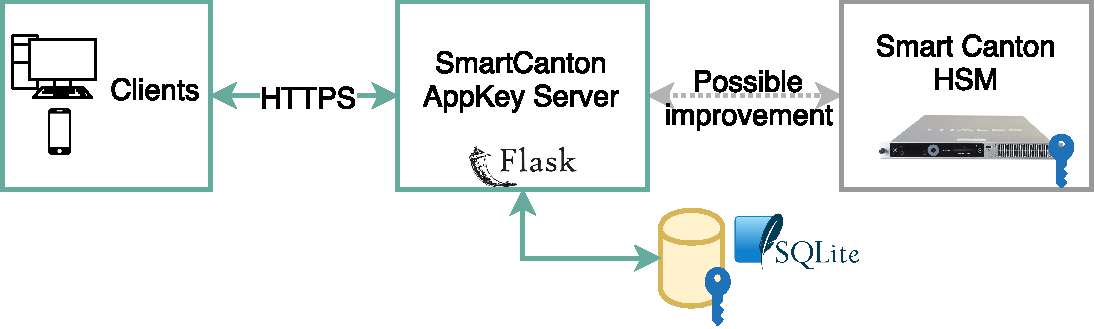
\includegraphics[width=1.0\textwidth]{Figures/Software/diagram_architecture_rest_api.pdf}
    \caption{Diagramme de communication entre les utilisateurs et le serveur de gestion des AppKey}
    \label{fig-diagram_architecture_rest_api}
\end{figure}

À l'heure actuelle, le serveur doit être provisionné manuellement avec les différentes AppKey dans sa base de données. Dans une vision plus finale du projet, il serait intéressant que le serveur ait accès au HSM lors de l'enregistrement du périphérique (lien \textit{possible improvement} sur la \cref{fig-diagram_architecture_rest_api}). Lorsque'un périphérique souhaite s'enregistrer sur le réseau, il demande la génération de sa clé AppKey via l'API REST du serveur, qui elle communique avec le HSM pour créer la clé. Ensuite, cette clé n'est plus stockée dans le serveur, mais directement transmisse au périphérique, afin que celui-ci puisse rejoindre le réseau. Ainsi, la seule copie de la clé est sur le périphérique et dans le HSM.

\subsection{Frameworks utilisés}

Python est un langage de programmation très riche en bibliothèques. Dans le cadre de l'implémentation de ce serveur, deux bibliothèques ont principalement été utilisées pour accélérer le processus de développement.

\subsubsection{Flask}
\label{sec-framework_flask}


Flask\footnote{\url{http://flask.pocoo.org/}} est un framework de développement web en Python. Son optique est d'être léger afin de laisser le maximum de souplesse liée à la programmation en Python \cite{Flaskfra59:online}. Plusieurs \textit{templates} sont également disponibles, de même que différentes extensions. Par exemple, pour les accès à la base de données, un sous module de Flask nommé Flask-SQLAlchemy\footnote{\url{http://flask-sqlalchemy.pocoo.org/2.3/}} a été utilisé pour faciliter les accès en écriture et en lecture à la base de données SQLite. \\


Une route d'accès à l'API peut être créée en quelques lignes en utilisant Flask. Voici par exemple comment afficher le message Hello World! à l'utilisateur se connectant à l'URL \url{http://127.0.0.1:5000/} (le port par défaut est 5000) :
\begin{tcolorbox}[top=-3mm, bottom=-3mm, left=0mm, right=0mm, enhanced, breakable, colback=LightGray, colframe=DarkGray, colbacktitle=DarkGray]
\begin{minted}[bgcolor=LightGray,fontsize=\footnotesize,breaklines]{python}
from flask import Flask
app = Flask(__name__)
 
@app.route("/")
def hello():
    return "Hello World!"
 
if __name__ == "__main__":
    app.run()
\end{minted}
\end{tcolorbox}


\subsubsection{Flask-JWT-Extended}


Le principe des JWT a été présenté en \cref{sec-security_jwt}. Plusieurs frameworks pour la génération et la vérification de ces \textit{tokens} ont été testés, il y eut tout d'abord \texttt{PyJWT}\footnote{\url{https://github.com/jpadilla/pyjwt}} et \texttt{python-jwt}\footnote{\url{https://github.com/davedoesdev/python-jwt}}. Le principal inconvénient de ces deux implémentations réside dans le fait qu'elles ne sont pas parfaitement adaptées pour fonctionner en tandem avec Flask. La validité du \textit{token} doit être traitée à l'intérieur du \textit{callback} défini par le décorateur de la route Flask (\texttt{@app.route}). Certaines autres bibliothèques ont donc été développées afin que le décorateur de flask appelle premièrement une fonction de validation du token. Les deux bibliothèques essayées ont été \texttt{FlaskJWT}\footnote{\url{https://github.com/mattupstate/flask-jwt}} et \texttt{Flask-JWT-Extended} \footnote{\url{https://github.com/vimalloc/flask-jwt-extended}}. Après plusieurs tests d'implémentation, il a été retenu que la bibliothèque \texttt{Flask-JWT-Extended} est beaucoup plus simple d'utilisation et contient plus de fonctionnalités. Elle est également beaucoup plus active en termes de développement. \texttt{FlaskJWT} ne dispose que de 99 \textit{commits} qui remontent à 2015, alors que \texttt{Flask-JWT-Extended} reçoit plusieurs \textit{commits} chaque mois. La documentation les étapes d'installation sont disponibles à l'adresse suivante :

\begin{center}
    \url{https://github.com/vimalloc/flask-jwt-extended}
\end{center}



\subsection{Base de données}



La structure de la base de données est visible sur la \cref{fig-database_model} avec la présence de deux tables nommées \path{user} et \path{smartcanton_devbox_device}. Le couple \path{ble_mac_addr} et \path{device_eui} est unique dans la table du device. Chaque périphérique est lié à un propriétaire à l'aide d'un ID unique autoincrémenté à l'ajout d'un utilisateur de la table \path{user}. Le mot de passe est stocké à l'aide d'un \textit{hash} généré avec l'algorithme sha256. Le champ \path{public_id} est l'identifiant UUID qui doit être utilisé lors des requêtes impliquant un utilisateur à l'API. Celui-ci est unique et permet de ce fait d'anonymiser le nom de l'utilisateur. Un administrateur, spécifié par le champ \texttt{admin}, a des privilèges spéciaux qui sont décrits en \cref{sec-software_serv_routes}.
Le \textit{passkey} Bluetooth n'est pas obligatoire, car certaines DevBox peuvent être installées sans ce mécanisme de sécurité, cependant cela n'est pas conseillé. \\

La base de données du serveur est stockée dans un fichier SQLite. Lors de la présentation de Flash en  \cref{sec-framework_flask}, celui-ci a été couplé avec le module SQLAlchemy qui facilite la création des tables, ainsi que l'accès à celles-ci depuis les différentes routes REST implémentées. Si l'utilisateur souhaite utiliser une autre base de données, SQLAlchemy peut reconstruire les tables simplement en lui spécifiant une nouvelle base de données. 

\begin{figure}[ht!]
    \centering
    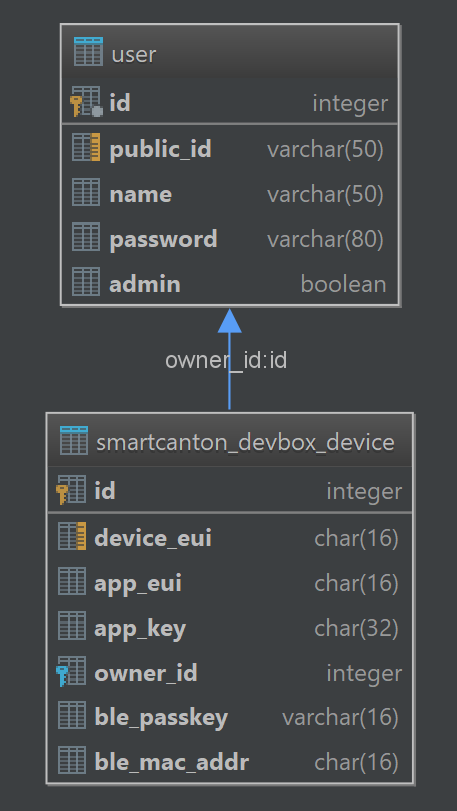
\includegraphics[width=0.4\textwidth]{Figures/Appendixes/database_model.PNG}
    \caption{Contenu de la base de données}
    \label{fig-database_model}
\end{figure}

\subsection{Routes REST}
\label{sec-software_serv_routes}

La documentation complète de l'API REST ainsi que des exemples sont disponibles en \cref{AppendixRestApiDoc} de ce document. Quatre types de requêtes disponibles sur les API REST ont été utilisées (\texttt{POST}, \texttt{GET}, \texttt{PUT} et \texttt{DELETE}). Une gestion des droits d'utilisateurs a également été respectée à l'aide du champ \texttt{admin} de la base de données. Voici un résumé des fonctionnalités qui ont été implémentées sur le serveur : 
\begin{itemize}
    \item {[\texttt{POST}]} Authentification de la paire nom d'utilisateur et mot de passe, puis si authentification acceptée, la génération d'un \textit{token} JWT en réponse;
    
    \item Gestion des utilisateurs : 
    \begin{enumerate}
        \item {[\texttt{GET}]} Lister tous les utilisateurs;
        \item {[\texttt{GET}]} Récupérer des informations détaillées sur un utilisateur précis;
        \item {[\texttt{PUT}]} Mise à jour des informations d'utilisateurs existants;
        \item {[\texttt{POST}]} Création de nouveaux utilisateurs;
        \item {[\texttt{DELETE}]} Suppression d'utilisateurs existants;
    \end{enumerate}
    
    \item Gestion des SmartCanton DevBox : 
    \begin{enumerate}
        \item {[\texttt{GET}]} Lister tous les périphériques DevBox;
        \item {[\texttt{GET}]} Récupérer des informations détaillées sur un périphérique précis;
        \item {[\texttt{PUT}]} Mise à jour des informations d'un périphérique existant;
        \item {[\texttt{POST}]} Création de nouvelles DevBox;
        \item {[\texttt{DELETE}]} Suppression des DevBox existantes.\\
    \end{enumerate}
\end{itemize}


Pour la gestion des utilisateurs, si le compte connecté n'est pas administrateur, alors il peut uniquement accéder, modifier et supprimer les informations le concernant. Par exemple, il ne peut lister que ses périphériques et non ceux de tout le réseau. Certaines fonctionnalités sont limitées seulement aux utilisateurs de types administrateurs, en voici la liste : 
\begin{itemize}
    \item Modification des mots de passe des utilisateurs (ne peut pas consulter, uniquement modifier le \textit{hash}) ainsi que les diverses informations de n'importe quel utilisateur;
    \item Ajout de nouveaux utilisateurs;
    \item Promulguer un utilisateur (nouveau ou existant) au rang d'administrateur;
    \item Supprimer des utilisateurs. \\
\end{itemize}


Pour spécifier un périphérique DevBox, c'est le champ \path{ble_mac_addr} qui est utilisé, car c'est le seul élément que le smartphone peut lire sans avoir besoin de se connecter à la DevBox. La documentation en \cref{AppendixRestApiDoc} explique plus en détail les permissions pour chaque commande.



\subsection{Certificats SSL}

Puisqu'une application Android doit être développée dans ce projet pour accéder à des URLs en HTTPS, une condition doit être respectée. Il est impératif d'utiliser un serveur qui utilise des certificats qui sont signés par une autorité de certifications. Si ce n'est pas le cas, Android refuse d'accéder à une quelconque ressource provenant de ces URLs. Il est possible d'ajouter son propre certificat dans Android, mais c'est une tâche compliquée, qui n'est pas très agréable pour l'utilisateur. \\

Pour la génération des certificats SSL, on peut directement contacter des sociétés comme Verisign ou Comodo, moyennant une cotisation annuelle, ils peuvent prodiguer un certificat pour un nom de domaine désiré. Cependant, depuis le 12 avril 2016, l'autorité de certification nommée \textit{Let's Encrypt} offre la possibilité de générer des certificats gratuitement \cite{LetsEncr96:online}. \textit{Let's Encrypt} est un service fourni par l’\textit{Internet Security Research Group} (ISRG), financé par de grandes entreprises et associations. \\

L'utilisateur désirant un certificat SSL doit prouver qu'il a accès au port 80 ou 443 du serveur derrière un nom de domaine. Pour cela, un logiciel doit être exécuté sur le serveur pour d'utiliser un de ces deux ports. Le plus connu est CertBot\footnote{\url{https://certbot.eff.org/}}. Dans le cas de ce projet, le serveur Web est directement implémenté par Flask. Il faut donc générer les clés et ensuite les passés en paramètres dans le code. Mais si l'utilisateur utilise Apache ou Nginx comme serveur web, il existe des \textit{plug-ins} pour ceux-ci qui s'occupent de renouveler automatiquement le certificat. Celui-ci peut donc être généré avec la commande suivante :

\begin{tcolorbox}[top=-3mm, bottom=-3mm, left=0mm, right=0mm, enhanced, breakable, colback=LightGray, colframe=DarkGray, colbacktitle=DarkGray]
\begin{minted}[bgcolor=LightGray,fontsize=\footnotesize,breaklines]{bash}
$ sudo certbot certonly --standalone --preferred-challenges http -d lsn.eig.ch
\end{minted}
\end{tcolorbox}


Tous les 3 mois, cette commande doit être réexcutée afin que le service n'invalide pas le sous domaine. Les fichiers généré peuvent être listés à l'aide de la commande suivante : 

\begin{tcolorbox}[top=-3mm, bottom=-3mm, left=0mm, right=0mm, enhanced, breakable, colback=LightGray, colframe=DarkGray, colbacktitle=DarkGray]
\begin{minted}[bgcolor=LightGray,fontsize=\footnotesize,breaklines]{text}
$ certbot certificates
Saving debug log to /var/log/letsencrypt/letsencrypt.log
----------------------------------------------------------------------------
Found the following certs:
  Certificate Name: lsn.eig.ch
    Domains: lsn.eig.ch
    Expiry Date: 2018-03-20 12:11:40+00:00 (VALID: 89 days)
    Certificate Path: /etc/letsencrypt/live/lsn.eig.ch/fullchain.pem
    Private Key Path: /etc/letsencrypt/live/lsn.eig.ch/privkey.pem
----------------------------------------------------------------------------
\end{minted}
\end{tcolorbox}

Ceux-ci doivent être passés en paramètres à Flask afin de mettre en place des connexions HTTPS : 
\begin{tcolorbox}[top=-3mm, bottom=-3mm, left=0mm, right=0mm, enhanced, breakable, colback=LightGray, colframe=DarkGray, colbacktitle=DarkGray]
\begin{minted}[bgcolor=LightGray,fontsize=\footnotesize,breaklines]{python}
context = ssl.SSLContext(ssl.PROTOCOL_TLSv1_2)
chain_path = 'ssl_certificates/fullchain.pem'
chain_path = os.path.join(os.path.dirname(__file__), chain_path)
privkey_path = 'ssl_certificates/privkey.pem'
privkey_path = os.path.join(os.path.dirname(__file__), privkey_path)
context.load_cert_chain(chain_path, privkey_path)
\end{minted}
\end{tcolorbox}




